\documentclass[12pt,a4paper]{article}
\usepackage[a4paper, margin=0.8in, headheight=14pt]{geometry}
\usepackage{fontspec}
\usepackage{unicode-math}
\setmainfont{TeX Gyre Pagella}
\setmonofont[Scale=0.88]{TeX Gyre Cursor}
\setmathfont{Latin Modern Math}
\usepackage{xcolor}
\usepackage{titlesec}
\usepackage{enumitem}
\usepackage{tabularx}
\usepackage{booktabs}
\usepackage{array}
\usepackage{amsmath}
\usepackage{tikz}
\usetikzlibrary{shapes.geometric, arrows.meta, positioning, calc, fit, decorations.pathreplacing}
\usepackage{tcolorbox}
\tcbuselibrary{skins, breakable}
\usepackage{hyperref}
\usepackage{fancyhdr}
\usepackage{graphicx}
\usepackage{microtype}
\hyphenpenalty=10000
\exhyphenpenalty=10000
\sloppy
\usepackage{caption}
\usepackage{setspace}
\usepackage{multirow}
\usepackage{tocloft}
\newcommand{\Q}[1]{\textbf{#1}\par\noindent\ignorespaces}
\definecolor{myred}{RGB}{196,30,58}
\definecolor{mydark}{RGB}{30,30,50}
\definecolor{mygreen}{RGB}{14,120,80}
\definecolor{myteal}{RGB}{0,130,140}
\definecolor{myamber}{RGB}{180,100,0}
\definecolor{mypurple}{RGB}{100,30,160}
\definecolor{mygray}{RGB}{246,247,249}
\definecolor{mgframe}{RGB}{180,185,200}
\definecolor{watermark}{RGB}{145,150,170}
\definecolor{hdrred}{RGB}{250,232,235}
\definecolor{hdrgreen}{RGB}{220,244,233}
\definecolor{hdrteal}{RGB}{220,242,244}
\definecolor{hdramber}{RGB}{253,242,215}
\definecolor{hdrpurple}{RGB}{238,228,255}
\definecolor{hdrgray}{RGB}{238,240,245}
\definecolor{rowalt}{RGB}{250,251,253}

\titleformat{\section}{\large\bfseries\color{myred}}{\thesection.}{0.5em}{}[\vspace{1pt}{\color{myred}\rule{\linewidth}{0.8pt}}]
\titleformat{\subsection}{\normalsize\bfseries\color{myteal}}{\thesubsection}{0.5em}{}
\titlespacing*{\section}{0pt}{18pt}{7pt}
\titlespacing*{\subsection}{0pt}{11pt}{4pt}
\setlength{\parindent}{0pt}
\setlength{\parskip}{4pt}
\renewcommand{\cfttoctitlefont}{\large\bfseries\color{myred}}
\renewcommand{\cftaftertoctitle}{\par\noindent{\color{myred}\rule{\linewidth}{0.8pt}}}
\setlength{\cftbeforetoctitleskip}{0pt}
\setlength{\cftaftertoctitleskip}{6pt}
\renewcommand{\cftsecfont}{\normalsize\bfseries\color{mydark}}
\renewcommand{\cftsecpagefont}{\normalsize\bfseries\color{mydark}}
\renewcommand{\cftsecleader}{\cftdotfill{\cftdotsep}}
\setlength{\cftbeforesecskip}{7pt}
\renewcommand{\cftsubsecfont}{\small\color{mydark}}
\renewcommand{\cftsubsecpagefont}{\small\color{mydark}}
\setlength{\cftbeforesubsecskip}{3pt}
\setlength{\cftsubsecindent}{1.4em}
\renewcommand{\cftpartfont}{\normalsize\bfseries\color{myteal}}
\renewcommand{\cftpartpagefont}{\normalsize\bfseries\color{myteal}}
\setlength{\cftbeforepartskip}{14pt}
\renewcommand{\arraystretch}{1.45}
\setlength{\tabcolsep}{6pt}
\newcolumntype{B}[1]{>{\small\bfseries\raggedright\arraybackslash}m{#1}}
\newcolumntype{C}[1]{>{\centering\arraybackslash}m{#1}}
\newcolumntype{Y}{>{\small\raggedright\arraybackslash}X}
\renewcommand{\tabularxcolumn}[1]{m{#1}}
\newcommand{\currmodule}{Module 1}
\pagestyle{fancy}
\fancyhf{}
\fancyhead[L]{\small\color{myred}\textbf{PE-EC603D}\;\color{mydark}--- Information Theory and Coding}
\fancyhead[R]{\small\color{myteal}\textbf{\currmodule\ Notes}}
\fancyfoot[C]{\small\color{mydark}\thepage}
\fancyfoot[R]{\small\color{watermark}\textit{\copyright\ Biraj}}
\renewcommand{\headrulewidth}{0.5pt}
\renewcommand{\footrulewidth}{0.3pt}

\hypersetup{colorlinks=true, linkcolor=myteal, urlcolor=myteal,
  pdfauthor={Biraj Sarkar},
  pdftitle={PE-EC603D --- Combined Notes}}

\tcbset{
  tikzbox/.style={
    colback=mygray, colframe=mgframe, boxrule=0.6pt, arc=4pt,
    left=8pt, right=8pt, top=6pt, bottom=6pt,
    colbacktitle=mgframe, coltitle=mydark,
    fonttitle=\small\bfseries
  },
  defbox/.style={
    colback=hdrgreen, colframe=mygreen, boxrule=0.8pt, arc=4pt,
    left=9pt, right=9pt, top=6pt, bottom=6pt,
    colbacktitle=mygreen, coltitle=white,
    fonttitle=\small\bfseries
  },
  formulabox/.style={
    colback=hdrteal, colframe=myteal, boxrule=0.8pt, arc=4pt,
    left=9pt, right=9pt, top=7pt, bottom=7pt,
    colbacktitle=myteal, coltitle=white,
    fonttitle=\small\bfseries
  },
  examplebox/.style={
    colback=hdramber, colframe=myamber, boxrule=0.8pt, arc=4pt,
    left=9pt, right=9pt, top=6pt, bottom=6pt,
    colbacktitle=myamber, coltitle=white,
    fonttitle=\small\bfseries
  },
  masonbox/.style={
    colback=hdrpurple, colframe=mypurple, boxrule=0.8pt, arc=4pt,
    left=9pt, right=9pt, top=6pt, bottom=6pt,
    colbacktitle=mypurple, coltitle=white,
    fonttitle=\small\bfseries
  },
  exambox/.style={
    colback=hdrpurple, colframe=mypurple, boxrule=1pt, arc=5pt,
    left=10pt, right=10pt, top=8pt, bottom=8pt,
    colbacktitle=mypurple, coltitle=white,
    fonttitle=\bfseries,
    breakable, title after break={\textbf{Frequently Asked / Viva Questions (contd.)}}}
}
\tcbset{breakable}

\tikzset{
  block/.style={rectangle, draw=myteal, fill=hdrteal,
    text width=2.4cm, align=center, minimum height=0.95cm,
    font=\small, rounded corners=3pt, line width=0.7pt},
  redblock/.style={rectangle, draw=myred, fill=hdrred,
    text width=2.4cm, align=center, minimum height=0.95cm,
    font=\small, rounded corners=3pt, line width=0.7pt},
  netnode/.style={rectangle, draw=myteal, fill=hdrteal,
    text width=1.5cm, align=center, minimum height=0.8cm,
    font=\small, rounded corners=3pt, line width=0.7pt},
  sumjunc/.style={circle, draw=myamber, fill=hdramber,
    minimum size=0.62cm, font=\small, line width=0.8pt},
  snode/.style={circle, draw=mypurple, fill=hdrpurple,
    minimum size=0.55cm, font=\footnotesize, line width=0.7pt},
  arrow/.style={-Stealth, thick, color=mydark},
  redarrow/.style={-Stealth, thick, color=myred},
  line/.style={thick, color=mydark}
}

\newcommand{\modulestart}[2]{%
  \clearpage
  \renewcommand{\currmodule}{Module #1}%
  \phantomsection
  \addcontentsline{toc}{part}{Module #1: #2}%
  \setcounter{section}{0}%
  \begin{center}
    \vspace*{1.0cm}
    {\Huge\bfseries\color{myred} Module #1}\\[10pt]
    {\Large\bfseries\color{mydark} #2}\\[10pt]
    {\color{myred}\rule{0.55\linewidth}{1.2pt}}
  \end{center}
  \vspace{14pt}
}
\begin{document}

\thispagestyle{empty}
\vspace*{1.0cm}
\begin{center}
  {\Huge\bfseries\color{myred} PE-EC603D}\\[10pt]
  {\LARGE\bfseries\color{mydark} Information Theory and Coding}\\[20pt]
  {\color{myred}\rule{0.7\linewidth}{1.5pt}}\\[18pt]
  {\Large\color{myteal}\textbf{Combined Module Notes}}\\[8pt]
  {\large\color{mydark} Modules 1 -- 3}\\[40pt]
  {\normalsize\color{mydark} Semester VI \quad$\bullet$\quad 3L:0T:0P \quad$\bullet$\quad 3 Credits}\\[12pt]
  {\normalsize\color{mydark} CGEC \;$|$\; B.Tech ECE (2023--27)}\\[6pt]
  {\normalsize\color{mydark}\textit{Biraj Sarkar}}
\end{center}
\vspace{1.0cm}
\begin{center}
  \begin{tcolorbox}[colback=mygray, colframe=mgframe, boxrule=0.5pt, arc=3pt, width=0.85\linewidth]
    \centering\small\color{mydark}
    \textbf{Disclaimer / Study Guide Notice:}\\
    These are condensed \textbf{Short Notes} focusing on core theory, key formulas, block/circuit diagrams, and standard viva Q\&As for university exam revision. Exhaustive numerical practice problems and derivation edge cases are not covered. This serves as a quick-revision reference guide for students.
  \end{tcolorbox}
\end{center}
\vfill
\begin{center}{\small\color{watermark}\textit{Exam-Ready Notes}}\end{center}
\clearpage

\hypersetup{linkcolor=mydark}
\tableofcontents
\hypersetup{linkcolor=myteal}
\clearpage

% -- Module 1 -----------------------------------------------------------------
\modulestart{1}{Basics of Information Theory}

\section{Basics of Information Theory}
% ===============================================================================

Information theory is a mathematical framework developed by Claude Shannon in 1948 to quantify, store, and communicate digital information. It defines limits on data compression and transmission rates.

\subsection{Model of a Digital Communication System}
Before quantifying information, we analyze the basic blocks involved in its transmission:

\begin{tcolorbox}[tikzbox, title={Block Diagram of a Digital Communication System}]
\centering
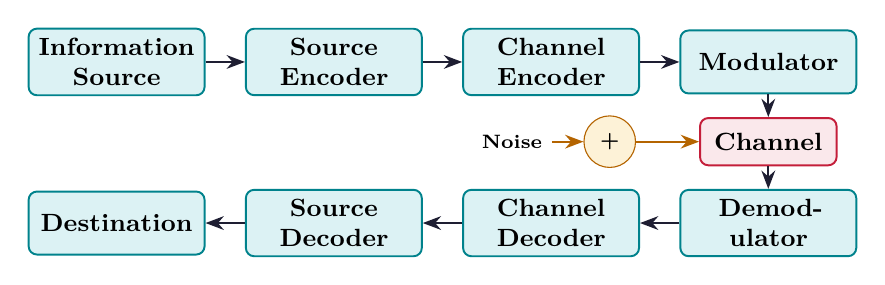
\begin{tikzpicture}[node distance=0.35cm and 0.55cm,
  sblock/.style={rectangle, draw=myteal, fill=hdrteal, text width=2.0cm,
    align=center, minimum height=0.8cm, font=\small\bfseries,
    rounded corners=3pt, line width=0.7pt}]
  
  % Row 1: Transmitter side
  \node[sblock] (src) {Information Source};
  \node[sblock, right=0.5cm of src] (senc) {Source Encoder};
  \node[sblock, right=0.5cm of senc] (cenc) {Channel Encoder};
  \node[sblock, right=0.5cm of cenc] (mod) {Modulator};
  
  % Row 2: Receiver side
  \node[sblock, below=1.2cm of mod] (demod) {Demodulator};
  \node[sblock, left=0.5cm of demod] (cdec) {Channel Decoder};
  \node[sblock, left=0.5cm of cdec] (sdec) {Source Decoder};
  \node[sblock, left=0.5cm of sdec] (dest) {Destination};

  % Middle block: Channel
  \path (mod.south) -- (demod.north) coordinate[midway] (chan_mid);
  \node[sblock, draw=myred, fill=hdrred, text width=1.5cm, minimum height=0.6cm] (chan) at (chan_mid) {Channel};

  % Arrows Row 1
  \draw[arrow] (src) -- (senc);
  \draw[arrow] (senc) -- (cenc);
  \draw[arrow] (cenc) -- (mod);
  \draw[arrow] (mod) -- (chan);

  % Arrows Row 2
  \draw[arrow] (chan) -- (demod);
  \draw[arrow] (demod) -- (cdec);
  \draw[arrow] (cdec) -- (sdec);
  \draw[arrow] (sdec) -- (dest);

  % Noise addition to channel
  \node[draw=myamber, fill=hdramber, circle, minimum size=0.4cm, left=0.8cm of chan, font=\scriptsize\bfseries] (sum) {+};
  \node[font=\scriptsize\bfseries, left=0.4cm of sum] (noise) {Noise};
  \draw[arrow, color=myamber] (noise) -- (sum);
  \draw[arrow, color=myamber] (sum) -- (chan);
\end{tikzpicture}
\end{tcolorbox}

\subsection{Measure of Information Content}
The "information" in a message is not related to its semantic meaning, but rather to its \textbf{uncertainty} or \textbf{surprise value}. An event that is highly likely to happen carries very little information when it occurs, whereas an extremely rare (unlikely) event carries high information.

\begin{tcolorbox}[defbox]
\textbf{Information Content:} The quantitative measure of the uncertainty associated with the occurrence of an event. For a discrete source emitting a symbol $x_i$ with probability $P(x_i)$, the information content $I(x_i)$ is inversely proportional to $P(x_i)$.
\end{tcolorbox}

\begin{tcolorbox}[formulabox, title={\textbf{Information Measurement Formula}}]
The information content $I(x_i)$ of symbol $x_i$ is defined as:
\begin{equation}
  I(x_i) = \log_r \left( \frac{1}{P(x_i)} \right) = -\log_r P(x_i)
\end{equation}
The unit of measurement depends on the base $r$ of the logarithm:
\begin{itemize}[leftmargin=1.5em, itemsep=2pt, topsep=2pt]
  \item[] \textbf{Base $r = 2$:} Units are \textbf{Bits} (Binary digits). $I(x_i) = -\log_2 P(x_i)$.
  \item[] \textbf{Base $r = e$:} Units are \textbf{Nats} (Natural units). $I(x_i) = -\ln P(x_i)$.
  \item[] \textbf{Base $r = 10$:} Units are \textbf{Hartleys} (or Decits). $I(x_i) = -\log_{10} P(x_i)$.
\end{itemize}
\textbf{Conversion Relations:}
\begin{align}
  1 \text{ Nat} &= \log_2 e \approx 1.443 \text{ Bits} \\
  1 \text{ Hartley} &= \log_2 10 \approx 3.322 \text{ Bits}
\end{align}
\end{tcolorbox}

\subsection{Entropy for Discrete Ensembles}
A discrete information source emits symbols from an alphabet $X = \{x_1, x_2, \dots, x_M\}$ with corresponding probabilities $P = \{P(x_1), P(x_2), \dots, P(x_M)\}$, where $\sum_{i=1}^M P(x_i) = 1$.

\begin{tcolorbox}[defbox]
\textbf{Entropy $H(X)$:} The average information content per symbol emitted by the source. It represents the mathematical expectation of the information of all symbols, measuring the overall uncertainty of the source.
\end{tcolorbox}

\begin{tcolorbox}[formulabox, title={\textbf{Entropy Formula}}]
\begin{equation}
  H(X) = E[I(x_i)] = \sum_{i=1}^M P(x_i) I(x_i) = -\sum_{i=1}^M P(x_i) \log_2 P(x_i) \quad (\text{bits/symbol})
\end{equation}
\end{tcolorbox}

\subsection{Properties of Entropy}
Entropy exhibits several fundamental properties that reflect its nature as a measure of uncertainty:

\begin{enumerate}[label=\textbf{\arabic*.}, leftmargin=*, itemsep=4pt]
  \item \textbf{Non-negativity:} $H(X) \ge 0$. Since $0 \le P(x_i) \le 1$, the term $-P(x_i) \log_2 P(x_i)$ is always non-negative.
  \item \textbf{Certainty (Minimum Entropy):} $H(X) = 0$ if and only if $P(x_i) = 1$ for some symbol $x_i$, and $P(x_j) = 0$ for all $j \ne i$. In this case, there is no uncertainty in the source output.
  \item \textbf{Maximality (Maximum Entropy):} $H(X) \le \log_2 M$, where $M$ is the number of symbols in the alphabet. The maximum uncertainty occurs when all symbols are equiprobable, i.e., $P(x_i) = 1/M$ for all $i$.
\end{enumerate}

\subsubsection{Derivation of Maximum Entropy Condition (Proof of Maximality)}
To find the probability distribution that maximizes $H(X)$ subject to the constraint $\sum_{i=1}^M P(x_i) = 1$, we use the method of Lagrange multipliers.
Let the objective function be:
\begin{equation*}
  f(P_1, P_2, \dots, P_M) = -\sum_{i=1}^M P_i \ln P_i
\end{equation*}
Subject to the constraint:
\begin{equation*}
  g(P_1, P_2, \dots, P_M) = \sum_{i=1}^M P_i - 1 = 0
\end{equation*}
Define the Lagrangian function $J$:
\begin{equation*}
  J = -\sum_{i=1}^M P_i \ln P_i - \lambda \left(\sum_{i=1}^M P_i - 1\right)
\end{equation*}
Differentiating $J$ with respect to $P_i$ and setting it to 0 for maximum value:
\begin{align*}
  \frac{\partial J}{\partial P_i} = - \ln P_i - 1 - \lambda &= 0 \\
  \ln P_i &= -(1 + \lambda) \\
  P_i &= e^{-(1+\lambda)}
\end{align*}
Since the right-hand side is constant and does not depend on the index $i$, all $P_i$ must be equal:
\begin{equation*}
  P_1 = P_2 = \dots = P_M = C \quad (\text{a constant})
\end{equation*}
Using the constraint $\sum_{i=1}^M P_i = 1$:
\begin{equation*}
  M \times C = 1 \implies C = \frac{1}{M} \implies P_i = \frac{1}{M} \quad \text{for all } i.
\end{equation*}
Substituting $P_i = 1/M$ back into the entropy formula yields the maximum entropy:
\begin{equation*}
  H(X)_{\text{max}} = -\sum_{i=1}^M \frac{1}{M} \log_2 \left(\frac{1}{M}\right) = -M \left(\frac{1}{M}\right) \left(-\log_2 M\right) = \log_2 M \quad \text{(Q.E.D.)}
\end{equation*}

\subsection{Binary Entropy Function}
For a binary source with alphabet $X = \{0, 1\}$ and probabilities $P(0) = p$ and $P(1) = 1-p$, the entropy is denoted by $H(p)$ or $H_b(p)$:
\begin{equation}
  H(p) = -p \log_2 p - (1-p) \log_2 (1-p)
\end{equation}

\begin{tcolorbox}[tikzbox, title={Binary Entropy Function $H(p)$ vs $p$}]
\centering
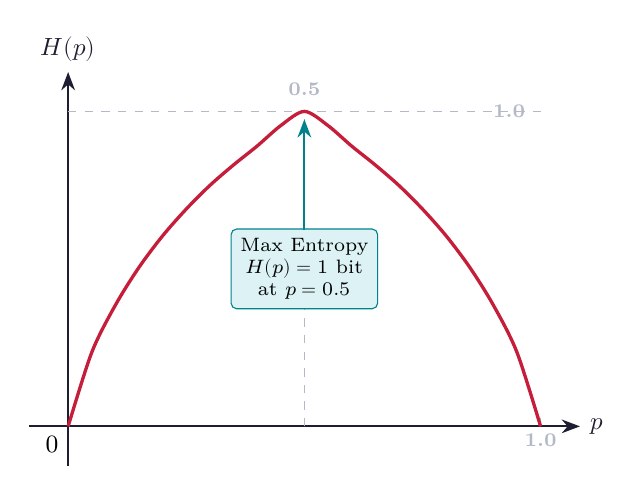
\begin{tikzpicture}
  % Draw axes
  \draw[-Stealth, thick, color=mydark] (-0.5,0) -- (6.5,0) node[right, font=\small] {$p$};
  \draw[-Stealth, thick, color=mydark] (0,-0.5) -- (0,4.5) node[above, font=\small] {$H(p)$};

  % Draw grid lines
  \draw[dashed, color=mgframe] (3,0) -- (3,4) node[above=2pt, font=\scriptsize\bfseries\color{mydark}] {0.5};
  \draw[dashed, color=mgframe] (0,4) -- (6,4) node[left=2pt, font=\scriptsize\bfseries\color{mydark}] {1.0};
  \draw[dashed, color=mgframe] (6,0) -- (6,0.1) node[below=2pt, font=\scriptsize\bfseries\color{mydark}] {1.0};

  % Plot the curve (manually plotting key points to avoid floating-point log domain errors)
  % Coordinates scaled: p=0 -> x=0, p=1 -> x=6; H(p)=0 -> y=0, H(p)=1 -> y=4
  \draw[very thick, color=myred, smooth] plot coordinates {
    (0.00, 0.00) (0.30, 0.94) (0.60, 1.54) (0.90, 2.02) (1.20, 2.42)
    (1.50, 2.76) (1.80, 3.06) (2.10, 3.32) (2.40, 3.56) (2.70, 3.82)
    (3.00, 4.00)
    (3.30, 3.82) (3.60, 3.56) (3.90, 3.32) (4.20, 3.06) (4.50, 2.76)
    (4.80, 2.42) (5.10, 2.02) (5.40, 1.54) (5.70, 0.94) (6.00, 0.00)
  };

  % Labels
  \node[below left, font=\small] at (0,0) {0};
  \node[draw=myteal, fill=hdrteal, rounded corners=2pt, font=\scriptsize, align=center] at (3,2) {Max Entropy\\$H(p) = 1$ bit\\at $p=0.5$};
  \draw[arrow, color=myteal] (3,2.5) -- (3,3.9);
\end{tikzpicture}
\end{tcolorbox}

% ===============================================================================
\section{Joint, Conditional, and Mutual Information}
% ===============================================================================

To analyze communication systems with an input source $X$ and an output destination $Y$, we define joint and conditional entropy metrics over the joint ensemble $(X, Y)$.

\subsection{Definitions of Entropies}
Let $P(x_i)$ be input probabilities, $P(y_j)$ be output probabilities, and $P(x_i, y_j)$ be the joint probability of transmitting $x_i$ and receiving $y_j$.

\begin{tcolorbox}[formulabox, title={\textbf{Joint and Conditional Entropies}}]
\begin{enumerate}[label=\textbf{\arabic*.}, leftmargin=1.5em, itemsep=4pt, topsep=2pt]
  \item \textbf{Joint Entropy $H(X, Y)$:} The total average uncertainty of the combined system.
    \begin{equation}
      H(X, Y) = -\sum_{i=1}^M \sum_{j=1}^N P(x_i, y_j) \log_2 P(x_i, y_j)
    \end{equation}
  \item \textbf{Conditional Entropy $H(X|Y)$:} The average uncertainty about the input $X$ after the output $Y$ is observed (also called \textbf{Equivocation}).
    \begin{equation}
      H(X|Y) = -\sum_{i=1}^M \sum_{j=1}^N P(x_i, y_j) \log_2 P(x_i|y_j)
    \end{equation}
  \item \textbf{Conditional Entropy $H(Y|X)$:} The average uncertainty about the output $Y$ when the input $X$ is known (represents the noise introduced by the channel).
    \begin{equation}
      H(Y|X) = -\sum_{i=1}^M \sum_{j=1}^N P(x_i, y_j) \log_2 P(y_j|x_i)
    \end{equation}
\end{enumerate}
\end{tcolorbox}

\subsubsection{Derivation of Joint Entropy Relations}
We derive the relation $H(X, Y) = H(X) + H(Y|X)$ using joint and conditional probability relationships $P(x_i, y_j) = P(x_i) P(y_j|x_i)$:
\begin{align*}
  H(X, Y) &= -\sum_{i=1}^M \sum_{j=1}^N P(x_i, y_j) \log_2 P(x_i, y_j) \\
  &= -\sum_{i=1}^M \sum_{j=1}^N P(x_i, y_j) \log_2 \left[ P(x_i) P(y_j|x_i) \right] \\
  &= -\sum_{i=1}^M \sum_{j=1}^N P(x_i, y_j) \left[ \log_2 P(x_i) + \log_2 P(y_j|x_i) \right] \\
  &= -\sum_{i=1}^M \left( \sum_{j=1}^N P(x_i, y_j) \right) \log_2 P(x_i) - \sum_{i=1}^M \sum_{j=1}^N P(x_i, y_j) \log_2 P(y_j|x_i)
\end{align*}
Using the probability marginalization rule $\sum_{j=1}^N P(x_i, y_j) = P(x_i)$:
\begin{equation*}
  H(X, Y) = -\sum_{i=1}^M P(x_i) \log_2 P(x_i) + H(Y|X) = H(X) + H(Y|X) \quad \text{(Q.E.D.)}
\end{equation*}
Similarly, using $P(x_i, y_j) = P(y_j) P(x_i|y_j)$, we can prove:
\begin{equation}
  H(X, Y) = H(Y) + H(X|Y)
\end{equation}

\subsection{Mutual Information}
\begin{tcolorbox}[defbox]
\textbf{Mutual Information $I(X; Y)$:} The amount of information about the source $X$ that is obtained by observing the channel output $Y$. It measures the reduction in uncertainty of $X$ due to the knowledge of $Y$.
\end{tcolorbox}

\begin{tcolorbox}[formulabox, title={\textbf{Mutual Information Formulas}}]
\begin{equation}
  I(X; Y) = H(X) - H(X|Y) \quad (\text{bits/symbol})
\end{equation}
By symmetry and joint entropy relations, it can also be expressed as:
\begin{align}
  I(X; Y) &= H(Y) - H(Y|X) \\
  I(X; Y) &= H(X) + H(Y) - H(X, Y)
\end{align}
In terms of probabilities:
\begin{equation}
  I(X; Y) = \sum_{i=1}^M \sum_{j=1}^N P(x_i, y_j) \log_2 \left[ \frac{P(x_i, y_j)}{P(x_i)P(y_j)} \right]
\end{equation}
\end{tcolorbox}

\subsection{Properties of Mutual Information}
\begin{itemize}[leftmargin=*, itemsep=3pt]
  \item \textbf{Symmetry:} $I(X; Y) = I(Y; X)$. The channel output $Y$ carries the same amount of information about the input $X$ as the input $X$ carries about the output $Y$.
  \item \textbf{Non-negativity:} $I(X; Y) \ge 0$. The observation of $Y$ can never increase the uncertainty of $X$ on average.
  \item \textbf{Independence Condition:} $I(X; Y) = 0$ if and only if $X$ and $Y$ are statistically independent. In this case, receiving $Y$ provides no information about $X$.
  \item \textbf{Relation to Channel Capacity:} For deterministic, noiseless channels, conditional uncertainty vanishes, and $I(X; Y) = H(X)$.
\end{itemize}

\subsection{Entropy Relationship Diagram}
The relationships between all these entropy measures are summarized in the Venn diagram below:

\begin{tcolorbox}[tikzbox, title={Venn Diagram of Entropy Relationships}]
\centering
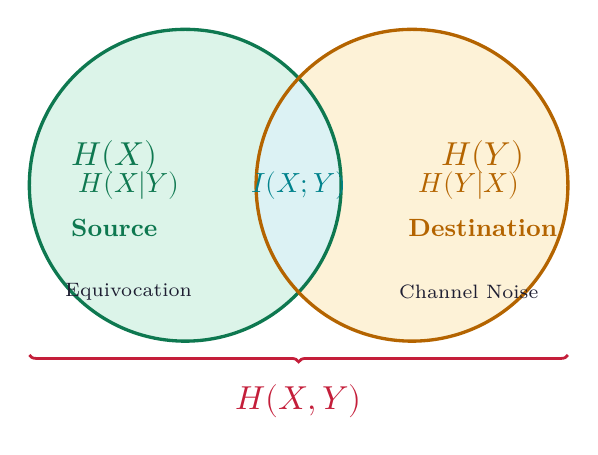
\begin{tikzpicture}[thick, scale=0.9]
  % Define overlapping circles
  \def\circleA{(-1.6,0) circle (2.2cm)}
  \def\circleB{(1.6,0) circle (2.2cm)}

  % Fill colors
  \begin{scope}
    \clip \circleA;
    \fill[hdrteal] \circleB; % Intersection (Mutual Info)
  \end{scope}

  \begin{scope}
    \clip \circleA;
    \fill[hdrgreen] \circleA;
    \clip \circleB;
    \fill[hdrteal] \circleA; % Redo intersection to keep clean
  \end{scope}
  
  \begin{scope}
    \clip \circleB;
    \fill[hdramber] \circleB;
    \clip \circleA;
    \fill[hdrteal] \circleB;
  \end{scope}

  % Draw outlines of circles
  \draw[mygreen, line width=1.2pt] \circleA;
  \draw[myamber, line width=1.2pt] \circleB;

  % Set labels
  \node[font=\large\bfseries\color{mygreen}] at (-2.6, 0.4) {$H(X)$};
  \node[font=\large\bfseries\color{myamber}] at (2.6, 0.4) {$H(Y)$};

  \node[font=\small\bfseries\color{mygreen}] at (-2.6, -0.6) {Source};
  \node[font=\small\bfseries\color{myamber}] at (2.6, -0.6) {Destination};

  % Labels inside divisions
  \node[font=\normalsize\bfseries\color{mygreen}] at (-2.4, 0) {$H(X|Y)$};
  \node[font=\normalsize\bfseries\color{myamber}] at (2.4, 0) {$H(Y|X)$};
  \node[font=\normalsize\bfseries\color{myteal}] at (0, 0) {$I(X; Y)$};

  % Curly brace for joint entropy
  \draw[decoration={brace, mirror, raise=5pt}, decorate, color=myred, line width=1pt] 
    (-3.8,-2.2) -- (3.8,-2.2) node[midway, below=12pt, font=\large\bfseries\color{myred}] {$H(X, Y)$};

  % Details below
  \node[font=\scriptsize\color{mydark}] at (-2.4,-1.5) {Equivocation};
  \node[font=\scriptsize\color{mydark}] at (2.4,-1.5) {Channel Noise};
\end{tikzpicture}
\end{tcolorbox}

% ===============================================================================
\section{Shannon's First Theorem \& Source Coding}
% ===============================================================================

Source coding is the process of representing discrete source symbols with binary code words. The goal is to reduce data size by removing redundancy.

\subsection{Shannon's Noiseless Coding Theorem}
\begin{tcolorbox}[defbox]
\textbf{Shannon's First Theorem (Source Coding Theorem):} For a discrete memoryless source $X$ with entropy $H(X)$ (bits/symbol), the average codeword length $L$ (bits/symbol) for any uniquely decodable binary code is bounded by:
\begin{equation}
  L \ge H(X)
\end{equation}
By coding sequences of $N$ symbols at a time (block coding), the average code length per source symbol $L_N$ can be made arbitrarily close to $H(X)$ as $N \to \infty$:
\begin{equation}
  \lim_{N \to \infty} L_N = H(X)
\end{equation}
\end{tcolorbox}

\subsection{Performance Metrics of Source Codes}
For a source emitting symbols $s_i$ with probability $P(s_i)$ and assigned codeword length $l_i$ (in bits):
\begin{tcolorbox}[formulabox, title={\textbf{Average Length, Efficiency, and Redundancy}}]
\begin{enumerate}[label=\textbf{\arabic*.}, leftmargin=1.5em, itemsep=4pt, topsep=2pt]
  \item \textbf{Average Codeword Length ($L$):}
    \begin{equation}
      L = \sum_{i=1}^M P(s_i) l_i \quad (\text{bits/symbol})
    \end{equation}
  \item \textbf{Coding Efficiency ($\eta$):}
    \begin{equation}
      \eta = \frac{H(X)}{L} \times 100\%
    \end{equation}
  \item \textbf{Code Redundancy ($R$):}
    \begin{equation}
      R = 1 - \eta = 1 - \frac{H(X)}{L}
    \end{equation}
\end{enumerate}
\end{tcolorbox}

\subsection{Prefix Codes and Kraft-McMillan Inequality}
A code is \textbf{uniquely decodable} if any concatenated sequence of codewords can be decoded in only one way.
\begin{tcolorbox}[defbox]
\textbf{Prefix Code (Instantaneous Code):} A uniquely decodable code with the property that no codeword is a prefix of any other codeword. This allows a sequence to be decoded symbol-by-symbol instantaneously as it is received, without waiting for the end of the sequence.
\end{tcolorbox}

\begin{tcolorbox}[formulabox, title={\textbf{Kraft-McMillan Inequality}}]
A prefix code (or any uniquely decodable code) with alphabet size $D$ (usually binary, $D=2$) and codeword lengths $l_1, l_2, \dots, l_M$ exists if and only if:
\begin{equation}
  \sum_{i=1}^M D^{-l_i} \le 1
\end{equation}
For binary codes, this is:
\begin{equation}
  \sum_{i=1}^M 2^{-l_i} \le 1
\end{equation}
If the inequality is satisfied with equality ($\sum 2^{-l_i} = 1$), the code is called a \textbf{complete code} (no further codewords can be added without violating the prefix property).
\tcbset{colbacktitle=myteal, coltitle=white}
\end{tcolorbox}

\subsection{Shannon-Fano Coding Algorithm}
Shannon-Fano coding is a top-down algorithm to construct prefix codes. The procedure is:
\begin{enumerate}[label=\textbf{Step \arabic*:}, leftmargin=4.5em, itemsep=3pt]
  \item Sort the source symbols in descending order of their probabilities.
  \item Divide the sorted list of symbols into two subsets such that the sum of probabilities of the two subsets is as close to equal as possible.
  \item Assign binary code '0' to all symbols in the first (upper) subset and '1' to all symbols in the second (lower) subset.
  \item Recursively apply Steps 2 and 3 to each subset until each sub-sublist contains exactly one symbol.
  \item The codeword for each symbol is the sequence of 0s and 1s assigned to it from the root of divisions.
\end{enumerate}

\begin{tcolorbox}[examplebox, title={Worked Example: Shannon-Fano Coding}]
\textbf{Problem:} A discrete memoryless source emits 5 symbols $\{s_1, s_2, s_3, s_4, s_5\}$ with probabilities $P = \{0.35, 0.30, 0.20, 0.10, 0.05\}$. 
\begin{enumerate}[label=\alph*., leftmargin=*, itemsep=1pt, topsep=1pt]
  \item Construct a binary Shannon-Fano code.
  \item Calculate the entropy $H(X)$ of the source.
  \item Calculate the average codeword length $L$ and the efficiency $\eta$.
\end{enumerate}
\textbf{Solution:}

\textbf{(a) Code Construction Table:}\par\noindent
\begin{tabularx}{\linewidth}{|B{1.5cm}|Y|Y|Y|Y|B{2.2cm}|B{1.6cm}|}
\hline
\textbf{Symbol} & \textbf{Prob.} & \textbf{Stage 1} & \textbf{Stage 2} & \textbf{Stage 3} & \textbf{Codeword} & \textbf{Length ($l_i$)} \\
\hline
$s_1$ & 0.35 & 0 & 0 & & 00 & 2 \\
$s_2$ & 0.30 & 0 & 1 & & 01 & 2 \\
\hline
$s_3$ & 0.20 & 1 & 0 & & 10 & 2 \\
$s_4$ & 0.10 & 1 & 1 & 0 & 110 & 3 \\
$s_5$ & 0.05 & 1 & 1 & 1 & 111 & 3 \\
\hline
\end{tabularx}
\par\vspace{4pt}
\textit{Division Rationale:}
\begin{itemize}[leftmargin=*, itemsep=1pt]
  \item \textbf{Stage 1:} Split between $\{s_1, s_2\}$ (sum = 0.65) and $\{s_3, s_4, s_5\}$ (sum = 0.35). Difference is $0.30$. (Splitting between $s_1$ and others yields difference $0.35 - 0.65 = 0.30$, so both partitions are valid. Let's use the first).
  \item \textbf{Stage 2:} Split upper subset $\{s_1\}$ (0.35) and $\{s_2\}$ (0.30). Split lower subset $\{s_3\}$ (0.20) and $\{s_4, s_5\}$ (0.15).
  \item \textbf{Stage 3:} Split $\{s_4\}$ (0.10) and $\{s_5\}$ (0.05).
\end{itemize}

\textbf{(b) Source Entropy $H(X)$:}
\begin{align*}
  H(X) &= -\sum_{i=1}^5 P(s_i) \log_2 P(s_i) \\
  &= -[0.35\log_2 0.35 + 0.30\log_2 0.30 + 0.20\log_2 0.20 + 0.10\log_2 0.10 + 0.05\log_2 0.05] \\
  &= -[0.35(-1.5146) + 0.30(-1.7370) + 0.20(-2.3219) + 0.10(-3.3219) + 0.05(-4.3219)] \\
  &= -[-0.5301 - 0.5211 - 0.4644 - 0.3322 - 0.2161] = 2.0639 \text{ bits/symbol}
\end{align*}

\textbf{(c) Average Codeword Length $L$ and Efficiency $\eta$:}
\begin{align*}
  L &= \sum_{i=1}^5 P(s_i) l_i = (0.35 \times 2) + (0.30 \times 2) + (0.20 \times 2) + (0.10 \times 3) + (0.05 \times 3) \\
  &= 0.70 + 0.60 + 0.40 + 0.30 + 0.15 = 2.15 \text{ bits/symbol} \\[4pt]
  \eta &= \frac{H(X)}{L} \times 100\% = \frac{2.0639}{2.15} \times 100\% \approx 95.99\% \\[4pt]
  \text{Redundancy } R &= 1 - 0.9599 = 0.0401 \text{ or } 4.01\%
\end{align*}
\textbf{Kraft Inequality Verification:}
\begin{equation*}
  \sum_{i=1}^5 2^{-l_i} = 2^{-2} + 2^{-2} + 2^{-2} + 2^{-3} + 2^{-3} = 0.25 + 0.25 + 0.25 + 0.125 + 0.125 = 1.0 \le 1
\end{equation*}
The sum equals 1.0. This indicates that the code is prefix-free and is a complete code.
\end{tcolorbox}

% ===============================================================================
% MANDATORY QUICK REVISION PAGE
% ===============================================================================
\newpage
\begin{center}
  {\large\bfseries\color{myred} Quick Revision --- Module I}\\[3pt]
  {\small\color{mydark} Basics \& Source Coding $|$ PE-EC603D}
\end{center}
\noindent{\color{myred}\rule{\linewidth}{1.2pt}}
\vspace{4pt}

\begin{tcolorbox}[formulabox, title={\textbf{Key Formulas at a Glance}}]
\renewcommand{\arraystretch}{1.3}
\begin{tabularx}{\linewidth}{B{4.5cm} X}
Self-Information        & $I(x_i) = \log_2 \left( \frac{1}{P(x_i)} \right) = -\log_2 P(x_i)$ \\[4pt]
Entropy (Average Info)   & $H(X) = -\sum_{i=1}^M P(x_i) \log_2 P(x_i)$ \\[4pt]
Joint Entropy           & $H(X, Y) = -\sum \sum P(x_i, y_j) \log_2 P(x_i, y_j)$ \\[4pt]
Conditional Entropies   & $H(X|Y) = H(X, Y) - H(Y)$ \quad and \quad $H(Y|X) = H(X, Y) - H(X)$ \\[4pt]
Mutual Information      & $I(X; Y) = H(X) - H(X|Y) = H(Y) - H(Y|X)$ \\[4pt]
Average Code Length     & $L = \sum P(s_i) l_i$ \\[4pt]
Coding Efficiency       & $\eta = \frac{H(X)}{L} \times 100\%$ \\[4pt]
Kraft Inequality        & $\sum 2^{-l_i} \le 1 \quad (\text{For binary prefix codes})$
\end{tabularx}
\end{tcolorbox}

\begin{tcolorbox}[defbox, title={\textbf{One-Line Definitions}}]
\begin{itemize}[leftmargin=*, itemsep=2.5pt, topsep=0pt]
  \item \textbf{Information Content:} A measure of surprise or uncertainty of an event, dependent only on its probability.
  \item \textbf{Entropy:} The average uncertainty or information content per symbol emitted by a source.
  \item \textbf{Equivocation $H(X|Y)$:} The residual uncertainty of the input $X$ after output $Y$ is observed at the receiver.
  \item \textbf{Mutual Information:} The amount of information shared between the transmitter and receiver.
  \item \textbf{Prefix Code:} A code in which no codeword is a prefix of another, enabling instantaneous decoding.
  \item \textbf{Kraft Inequality:} A mathematical condition determining the existence of prefix codes for given lengths.
  \item \textbf{Source Coding Theorem:} Shannon's limit stating that average codeword length cannot be less than source entropy.
  \item \textbf{Redundancy:} The percentage of code space wasted by transmitting non-informative bits ($R = 1 - \eta$).
\end{itemize}
\end{tcolorbox}

\begin{tcolorbox}[exambox, title={\textbf{Frequently Asked / Viva Questions}}]
\begin{enumerate}[topsep=0pt, label=\textbf{Q\arabic*.}, itemsep=5pt]
  \item \Q{State the units of information and their conversion relations.}
    Bits (base 2), Nats (base $e$), and Hartleys (base 10). Conversions: $1 \text{ Nat} = 1.443 \text{ Bits}$; $1 \text{ Hartley} = 3.322 \text{ Bits}$.
  \item \Q{Under what condition is the entropy of a source maximized?}
    When all $M$ symbols of the source alphabet are equiprobable, i.e., $P(x_i) = 1/M$ for all $i$. The maximum entropy is $H(X)_{\text{max}} = \log_2 M$.
  \item \Q{What is the physical significance of conditional entropy $H(Y|X)$?}
    It represents the average uncertainty of the output $Y$ when the input $X$ is known. Physically, it measures the noise added by the channel.
  \item \Q{Explain the term "Equivocation" in communication channels.}
    Equivocation is $H(X|Y)$, which is the average uncertainty about the transmitted symbol $X$ after receiving symbol $Y$. It represents lost information.
  \item \Q{Why is Mutual Information symmetric?}
    $I(X; Y) = I(Y; X) = H(X) + H(Y) - H(X,Y)$. It represents the shared information between $X$ and $Y$, making the direction of analysis irrelevant.
  \item \Q{State Shannon's Source Coding Theorem.}
    The average length $L$ of any uniquely decodable binary code for a source $X$ satisfies $L \ge H(X)$. The minimum average code length is limited by the source entropy.
  \item \Q{What is an instantaneous code (prefix code)?}
    A code where no codeword is a prefix of any other codeword. It is decodable immediately upon receiving the last bit of the codeword, without looking ahead.
  \item \Q{What is the significance of the Kraft-McMillan Inequality?}
    It provides a necessary and sufficient condition for the existence of an instantaneous (prefix) code for a given set of codeword lengths.
  \item \Q{If a source has an entropy of $1.8$ bits/symbol and is encoded using a code with average length $2$ bits/symbol, find efficiency and redundancy.}
    Efficiency $\eta = \frac{1.8}{2} \times 100 = 90\%$. Redundancy $R = 100\% - 90\% = 10\%$.
  \item \Q{Why does block coding increase source coding efficiency?}
    Block coding groups $N$ symbols together, allowing the average length per symbol to approach the entropy $H(X)$ more closely as $N \to \infty$ by utilizing joint probabilities.
  \item \Q{Can the efficiency of a source code be greater than $100\%$?}
    No. According to Shannon's Source Coding Theorem, $L \ge H(X)$, meaning efficiency $\eta = H(X)/L \le 1.0$ (or $100\%$).
  \item \Q{State the main difference between Shannon-Fano and Huffman coding approaches.}
    Shannon-Fano is a top-down approach that partitions probabilities into subgroups, while Huffman coding is a bottom-up approach that recursively merges the lowest probabilities.
\end{enumerate}
\end{tcolorbox}

\begin{tcolorbox}[tikzbox, title={Comparison of Source Coding Techniques}]
\renewcommand{\arraystretch}{1.4}
\par\noindent
\begin{tabularx}{\linewidth}{|B{3.2cm}|Y|Y|}
\hline
\textbf{Parameter} & \textbf{\color{myteal}Fixed-Length Coding} & \textbf{\color{mygreen}Variable-Length Coding} \\
\hline
\textbf{Codeword Length} & Equal length ($l_i = \lceil \log_2 M \rceil$) for all symbols. & Different lengths based on symbol probabilities. \\
\hline
\textbf{Probability Sensitivity} & Ignores probability distribution. & Allocates shorter codes to high-probability symbols. \\
\hline
\textbf{Efficiency} & Low if symbols have unequal probabilities. & High (approaches Shannon's limit $H(X)$). \\
\hline
\textbf{Synchronization} & Easy; boundaries are known. & Harder; requires prefix-free property (Prefix codes). \\
\hline
\textbf{Examples} & ASCII, Standard PCM. & Shannon-Fano, Huffman coding. \\
\hline
\end{tabularx}
\end{tcolorbox}


% -- Module 2 -----------------------------------------------------------------
\modulestart{2}{Markov Sources}

\section{Markov Sources}
% ===============================================================================

Information sources are categorized based on whether current outputs depend on past outputs. A source is **memoryless** if symbols are emitted independently. A source has **memory** if current output probabilities are conditioned on previous symbols.

\subsection{Definition of Markov Sources}
\begin{tcolorbox}[defbox]
\textbf{Markov Source:} A discrete source with memory where the probability of emitting the next symbol depends on a finite number of preceding symbols.
\par\vspace{3pt}
In a **first-order Markov source**, the probability of the next symbol depends only on the immediately preceding symbol:
\begin{equation}
  P(S_t = s_j \mid S_{t-1} = s_i, S_{t-2} = s_k, \dots) = P(S_t = s_j \mid S_{t-1} = s_i) = p_{ij}
\end{equation}
Where $p_{ij}$ is the transition probability from state $s_i$ to state $s_j$.
\end{tcolorbox}

\begin{tcolorbox}[tikzbox, title={State Transition Diagram of a 2-State Markov Source}]
\centering
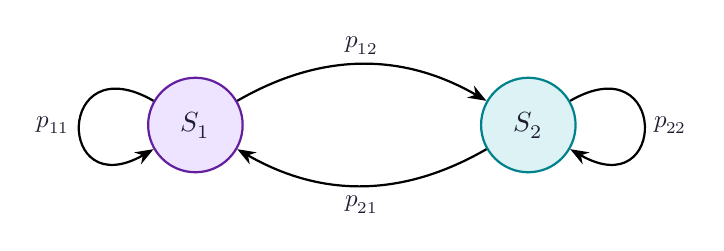
\begin{tikzpicture}[node distance=2.5cm,>=Stealth,auto,thick]
  % Nodes representing states
  \node[circle, draw=mypurple, fill=hdrpurple, minimum size=1.2cm, font=\bfseries\color{mydark}] (S1) {$S_1$};
  \node[circle, draw=myteal, fill=hdrteal, minimum size=1.2cm, right=3.0cm of S1, font=\bfseries\color{mydark}] (S2) {$S_2$};

  % Transition arrows
  \path[->] 
    (S1) edge [bend left=30] node[above, font=\small\color{mydark}] {$p_{12}$} (S2)
    (S2) edge [bend left=30] node[below, font=\small\color{mydark}] {$p_{21}$} (S1)
    (S1) edge [loop left, out=150, in=210, looseness=6] node[left, font=\small\color{mydark}] {$p_{11}$} (S1)
    (S2) edge [loop right, out=30, in=330, looseness=6] node[right, font=\small\color{mydark}] {$p_{22}$} (S2);
\end{tikzpicture}
\end{tcolorbox}

\subsection{Transition Probability Matrix (TPM)}
The transition probabilities of a Markov chain with $K$ states are organized into a square matrix $P$:
\begin{equation}
  P = \begin{bmatrix}
    p_{11} & p_{12} & \dots & p_{1K} \\
    p_{21} & p_{22} & \dots & p_{2K} \\
    \vdots & \vdots & \ddots & \vdots \\
    p_{K1} & p_{K2} & \dots & p_{KK}
  \end{bmatrix}
\end{equation}
Since the source must transition to one of the possible states, the sum of probabilities in each row is exactly 1:
\begin{equation}
  \sum_{j=1}^K p_{ij} = 1 \quad \text{for all } i = 1, 2, \dots, K
\end{equation}

\subsection{Stationary State Probabilities}
Let $\mathbf{W} = [w_1, w_2, \dots, w_K]$ represent the stationary (steady-state) probability vector, where $w_i$ is the probability that the source is in state $i$ in the long run.
\begin{tcolorbox}[formulabox, title={\textbf{Stationary State Probability Equations}}]
The stationary probability vector satisfies:
\begin{equation}
  \mathbf{W} P = \mathbf{W} \quad \text{and} \quad \sum_{i=1}^K w_i = 1
\end{equation}
Which yields a system of linear equations:
\begin{align}
  w_1 p_{11} + w_2 p_{21} + \dots + w_K p_{K1} &= w_1 \\
  w_1 p_{12} + w_2 p_{22} + \dots + w_K p_{K2} &= w_2 \\
  &\;\; \vdots \\
  w_1 + w_2 + \dots + w_K &= 1
\end{align}
\end{tcolorbox}

\subsection{Entropy of Markov Sources (Entropy Rate)}
Because the output probability depends on the current state, we first calculate the entropy of each state individually, and then compute the weighted average over all states.
\begin{tcolorbox}[formulabox, title={\textbf{Markov Source Entropy Rate Formulas}}]
\begin{enumerate}[label=\textbf{\arabic*.}, leftmargin=1.5em, itemsep=4pt, topsep=2pt]
  \item \textbf{Entropy of State $i$ ($H_i$):} The uncertainty of the next symbol given the source is currently in state $i$.
    \begin{equation}
      H_i = -\sum_{j=1}^K p_{ij} \log_2 p_{ij} \quad (\text{bits/symbol})
    \end{equation}
  \item \textbf{Average Entropy of Markov Source ($H(X)$):} The long-run average uncertainty per symbol.
    \begin{equation}
      H(X) = \sum_{i=1}^K w_i H_i = -\sum_{i=1}^K w_i \sum_{j=1}^K p_{ij} \log_2 p_{ij} \quad (\text{bits/symbol})
    \end{equation}
\end{enumerate}
\end{tcolorbox}

\begin{tcolorbox}[examplebox, title={Worked Example: Entropy Rate of a Markov Source}]
\textbf{Problem:} A 2-state Markov source has the following transition probability matrix:
\begin{equation*}
  P = \begin{bmatrix}
    0.8 & 0.2 \\
    0.3 & 0.7
  \end{bmatrix}
\end{equation*}
\begin{enumerate}[label=\alph*., leftmargin=*, itemsep=1pt, topsep=1pt]
  \item Find the stationary state probabilities $w_1$ and $w_2$.
  \item Calculate the state entropies $H_1$ and $H_2$.
  \item Find the average entropy rate $H(X)$ of this source.
\end{enumerate}
\textbf{Solution:}

\textbf{(a) Find stationary probabilities $w_1$ and $w_2$:}
Using $\mathbf{W}P = \mathbf{W}$:
\begin{equation*}
  [w_1, w_2] \begin{bmatrix} 0.8 & 0.2 \\ 0.3 & 0.7 \end{bmatrix} = [w_1, w_2]
\end{equation*}
This yields the equations:
\begin{align*}
  0.8w_1 + 0.3w_2 &= w_1 \implies 0.3w_2 = 0.2w_1 \implies w_2 = \frac{2}{3}w_1 \\
  0.2w_1 + 0.7w_2 &= w_2 \implies 0.2w_1 = 0.3w_2 \quad (\text{redundant})
\end{align*}
Using the probability normalization constraint $w_1 + w_2 = 1$:
\begin{equation*}
  w_1 + \frac{2}{3}w_1 = 1 \implies \frac{5}{3}w_1 = 1 \implies w_1 = 0.6 \quad \text{and} \quad w_2 = 0.4
\end{equation*}

\textbf{(b) Calculate state entropies $H_1$ and $H_2$:}
\begin{align*}
  H_1 &= -[0.8\log_2 0.8 + 0.2\log_2 0.2] = -[0.8(-0.3219) + 0.2(-2.3219)] = 0.7219 \text{ bits/symbol} \\
  H_2 &= -[0.3\log_2 0.3 + 0.7\log_2 0.7] = -[0.3(-1.7370) + 0.7(-0.5146)] = 0.8813 \text{ bits/symbol}
\end{align*}

\textbf{(c) Find the average entropy rate $H(X)$:}
\begin{align*}
  H(X) &= w_1 H_1 + w_2 H_2 \\
  &= (0.6 \times 0.7219) + (0.4 \times 0.8813) \\
  &= 0.4331 + 0.3525 = 0.7856 \text{ bits/symbol}
\end{align*}
\textbf{Answer:} $w_1=0.6, w_2=0.4$; $H_1=0.7219, H_2=0.8813$ bits/sym; average entropy is \textbf{0.7856 bits/symbol}.
\end{tcolorbox}

% ===============================================================================
\section{Shannon's Second Theorem (Noisy Channel Coding Theorem)}
% ===============================================================================

When transmitting data over physical media, noise corrupts signals, causing bit errors. Shannon proved that error-free communication is possible even over noisy channels, provided the transmission rate does not exceed a threshold called **Channel Capacity**.

\subsection{Channel Capacity Concept}
\begin{tcolorbox}[defbox]
\textbf{Channel Capacity ($C$):} The maximum rate at which information can be transmitted reliably through a communication channel. It is mathematically defined as the maximum of the mutual information $I(X; Y)$ over all possible input probability distributions $P(x)$:
\begin{equation}
  C = \max_{P(x)} I(X; Y) \quad (\text{bits/channel-use})
\end{equation}
\end{tcolorbox}

\subsection{Noisy Channel Coding Theorem}
\begin{tcolorbox}[exambox, title={\textbf{Shannon's Second Theorem (Noisy Channel Coding Theorem)}}]
Let a discrete memoryless channel have capacity $C$.
\begin{enumerate}[label=\textbf{\arabic*.}, leftmargin=1.5em, itemsep=3pt, topsep=1pt]
  \item \textbf{Theorem:} If the source transmission rate $R$ (bits/second) is less than or equal to $C$ ($R \le C$), there exists a coding scheme (with block length $N$ sufficiently large) such that the probability of error at the receiver, $P_e$, can be made arbitrarily small:
    \begin{equation}
      \lim_{N \to \infty} P_e = 0
    \end{equation}
  \item \textbf{Converse:} If $R > C$, it is impossible to design a coding scheme that achieves error-free transmission. The probability of bit error $P_e$ is bounded away from zero, and reliable communication cannot occur.
\end{enumerate}
\end{tcolorbox}

This theorem is historically significant because it proved that channel noise limits the **rate of transmission**, not its **accuracy**. We do not need noiseless channels for error-free data transfer; we only need appropriate error-correcting codes.

% ===============================================================================
\section{Calculation of Channel Capacity for Discrete Channels}
% ===============================================================================

A discrete channel is represented by input alphabet $X$, output alphabet $Y$, and a channel transition matrix containing conditional probabilities $P(y_j|x_i)$.

\subsection{Binary Symmetric Channel (BSC)}
The BSC is the most common model for binary transmission. The input and output alphabets are binary $\{0, 1\}$. The probability of a bit being transmitted correctly is $1-p$, and the probability of a bit being flipped (error) is $p$.

\begin{tcolorbox}[tikzbox, title={Binary Symmetric Channel (BSC) Transition Model}]
\centering
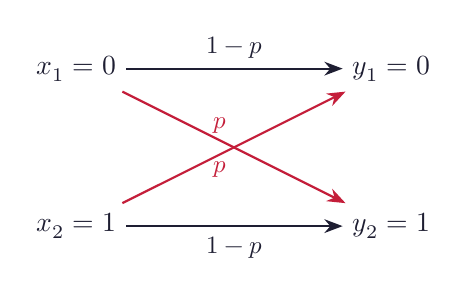
\begin{tikzpicture}[node distance=3.0cm, thick]
  % Inputs
  \node (X0) at (0, 2) [font=\bfseries\color{mydark}] {$x_1 = 0$};
  \node (X1) at (0, 0) [font=\bfseries\color{mydark}] {$x_2 = 1$};

  % Outputs
  \node (Y0) at (4, 2) [font=\bfseries\color{mydark}] {$y_1 = 0$};
  \node (Y1) at (4, 0) [font=\bfseries\color{mydark}] {$y_2 = 1$};

  % Transition arrows
  \draw[arrow] (X0) -- (Y0) node[midway, above, font=\small\color{myteal}] {$1-p$};
  \draw[arrow] (X1) -- (Y1) node[midway, below, font=\small\color{myteal}] {$1-p$};
  \draw[redarrow] (X0) -- (Y1) node[pos=0.3, right=5pt, font=\small\color{myred}] {$p$};
  \draw[redarrow] (X1) -- (Y0) node[pos=0.3, right=5pt, font=\small\color{myred}] {$p$};
\end{tikzpicture}
\tcbset{colbacktitle=myteal, coltitle=white}
\end{tcolorbox}

\subsubsection{Derivation of BSC Channel Capacity}
We calculate capacity using $I(X; Y) = H(Y) - H(Y|X)$.
First, evaluate the conditional entropy $H(Y|X)$:
\begin{align*}
  H(Y|X) &= -\sum_{i=1}^2 P(x_i) \sum_{j=1}^2 P(y_j|x_i) \log_2 P(y_j|x_i) \\
  &= -P(x_1) \left[ P(y_1|x_1)\log_2 P(y_1|x_1) + P(y_2|x_1)\log_2 P(y_2|x_1) \right] \\
  &\quad - P(x_2) \left[ P(y_1|x_2)\log_2 P(y_1|x_2) + P(y_2|x_2)\log_2 P(y_2|x_2) \right] \\
  &= -P(x_1) \left[ (1-p)\log_2(1-p) + p\log_2 p \right] - P(x_2) \left[ p\log_2 p + (1-p)\log_2(1-p) \right]
\end{align*}
Since $P(x_1) + P(x_2) = 1$:
\begin{equation*}
  H(Y|X) = -p\log_2 p - (1-p)\log_2(1-p) = H(p) \quad (\text{independent of input distribution } P(x))
\end{equation*}
Substitute this into the capacity equation:
\begin{equation*}
  C = \max_{P(x)} \left[ H(Y) - H(Y|X) \right] = \max_{P(x)} H(Y) - H(p)
\end{equation*}
Since $Y$ is a binary variable, its entropy $H(Y)$ is maximized when $Y$ has equiprobable outputs, i.e., $P(y_1) = P(y_2) = 0.5$, which yields $H(Y)_{\text{max}} = 1$. This maximum is achieved when the input symbols are equiprobable ($P(x_1) = P(x_2) = 0.5$).
\begin{tcolorbox}[formulabox, title={\textbf{BSC Channel Capacity}}]
\begin{equation}
  C_{\text{BSC}} = 1 - H(p) = 1 + p\log_2 p + (1-p)\log_2(1-p) \quad (\text{bits/channel-use})
\end{equation}
\end{tcolorbox}

\subsection{Binary Erasure Channel (BEC)}
In a BEC, the transmitter sends binary digits $\{0, 1\}$. Due to noise, the receiver may fail to decode the bit. Rather than receiving an incorrect bit, the receiver recognizes a lost bit and labels it as an erasure symbol '$e$'. The probability of erasure is $\alpha$.

\begin{tcolorbox}[tikzbox, title={Binary Erasure Channel (BEC) Transition Model}]
\centering
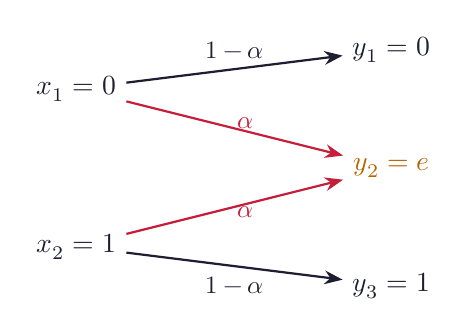
\begin{tikzpicture}[node distance=3.0cm, thick]
  % Inputs
  \node (X0) at (0, 2.5) [font=\bfseries\color{mydark}] {$x_1 = 0$};
  \node (X1) at (0, 0.5) [font=\bfseries\color{mydark}] {$x_2 = 1$};

  % Outputs
  \node (Y0) at (4, 3) [font=\bfseries\color{mydark}] {$y_1 = 0$};
  \node (Ye) at (4, 1.5) [font=\bfseries\color{myamber}] {$y_2 = e$};
  \node (Y1) at (4, 0) [font=\bfseries\color{mydark}] {$y_3 = 1$};

  % Transition arrows
  \draw[arrow] (X0) -- (Y0) node[midway, above, font=\small\color{myteal}] {$1-\alpha$};
  \draw[arrow] (X1) -- (Y1) node[midway, below, font=\small\color{myteal}] {$1-\alpha$};
  \draw[redarrow] (X0) -- (Ye) node[pos=0.4, right=5pt, font=\small\color{myred}] {$\alpha$};
  \draw[redarrow] (X1) -- (Ye) node[pos=0.4, right=5pt, font=\small\color{myred}] {$\alpha$};
\end{tikzpicture}
\tcbset{colbacktitle=myteal, coltitle=white}
\end{tcolorbox}

\subsubsection{Capacity of the BEC}
Let the input probability be $P(x=0) = \beta$, and $P(x=1) = 1-\beta$.
The output probabilities are:
\begin{align*}
  P(y=0) &= (1-\alpha)\beta \\
  P(y=e) &= \alpha\beta + \alpha(1-\beta) = \alpha \\
  P(y=1) &= (1-\alpha)(1-\beta)
\end{align*}
To find capacity, we compute conditional entropy $H(Y|X)$:
Since for any input $x$, the output is correct with probability $1-\alpha$ and erased with probability $\alpha$:
\begin{equation*}
  H(Y|X) = H(\alpha) = -\alpha \log_2 \alpha - (1-\alpha)\log_2(1-\alpha)
\end{equation*}
The output entropy $H(Y)$ is:
\begin{align*}
  H(Y) &= -P(y=0)\log_2 P(y=0) - P(y=e)\log_2 P(y=e) - P(y=1)\log_2 P(y=1) \\
  &= -(1-\alpha)\beta \log_2 \left[(1-\alpha)\beta\right] - \alpha\log_2 \alpha - (1-\alpha)(1-\beta)\log_2 \left[(1-\alpha)(1-\beta)\right] \\
  &= -\alpha\log_2 \alpha - (1-\alpha)\log_2(1-\alpha) + (1-\alpha)\left[ -\beta\log_2\beta - (1-\beta)\log_2(1-\beta) \right] \\
  &= H(\alpha) + (1-\alpha) H(X)
\end{align*}
Using $I(X; Y) = H(Y) - H(Y|X)$:
\begin{equation*}
  I(X; Y) = H(\alpha) + (1-\alpha)H(X) - H(\alpha) = (1-\alpha)H(X)
\end{equation*}
To maximize $I(X; Y)$, we maximize $H(X)$. Since $X$ is binary, its maximum entropy is $H(X)_{\text{max}} = 1$ bit (at $\beta = 0.5$).
\begin{tcolorbox}[formulabox, title={\textbf{BEC Channel Capacity}}]
\begin{equation}
  C_{\text{BEC}} = 1 - \alpha \quad (\text{bits/channel-use})
\end{equation}
\end{tcolorbox}
This shows that erasures reduce capacity linearly: if $20\%$ of bits are erased ($\alpha = 0.2$), the capacity is $80\%$ of a noiseless channel ($C = 0.8$ bits/use).

% ===============================================================================
\section{Application to Continuous Channels}
% ===============================================================================

Discrete channel models fail when signals are continuous voltage waveforms corrupted by additive white Gaussian noise (AWGN). We analyze these systems using continuous capacities.

\subsection{The Shannon-Hartley Theorem}
\begin{tcolorbox}[defbox]
\textbf{Shannon-Hartley Theorem:} The maximum rate of transmission over a continuous channel of bandwidth $B$ (Hz), corrupted by Additive White Gaussian Noise (AWGN) with signal power $S$ and noise power $N$, is:
\begin{equation}
  C = B \log_2 \left( 1 + \frac{S}{N} \right) \quad (\text{bits/second})
\end{equation}
\end{tcolorbox}
If noise spectral density is $N_0/2$ (double-sided) or $N_0$ (single-sided), the total noise power is $N = N_0 B$:
\begin{equation}
  C = B \log_2 \left( 1 + \frac{S}{N_0 B} \right)
\end{equation}

\subsection{Implications of Shannon-Hartley Theorem}
This relation highlights several trade-offs:
\begin{enumerate}[label=\textbf{\alph*.}, leftmargin=*, itemsep=3.5pt]
  \item \textbf{Signal-to-Noise Ratio (SNR) vs Bandwidth ($B$):} We can exchange bandwidth for SNR. A system with small bandwidth can achieve high capacity if the SNR is high, and vice-versa.
  \item \textbf{Infinite Bandwidth capacity limit:} If we keep signal power $S$ and noise density $N_0$ constant, and let the bandwidth $B$ grow to infinity, the capacity does not grow to infinity. Instead, it reaches a thermodynamic limit:
\end{enumerate}

\subsubsection{Derivation of Infinite Bandwidth Capacity}
We evaluate the limit of $C$ as $B \to \infty$:
\begin{equation*}
  \lim_{B \to \infty} C = \lim_{B \to \infty} B \log_2 \left( 1 + \frac{S}{N_0 B} \right)
\end{equation*}
Let $x = \frac{S}{N_0 B}$. As $B \to \infty$, $x \to 0$. We express $B$ as $B = \frac{S}{N_0 x}$:
\begin{align*}
  \lim_{B \to \infty} C &= \lim_{x \to 0} \frac{S}{N_0 x} \log_2 (1 + x) \\
  &= \frac{S}{N_0} \lim_{x \to 0} \log_2 (1 + x)^{1/x}
\end{align*}
By the definition of the natural base $e$, $\lim_{x \to 0} (1+x)^{1/x} = e$:
\begin{equation*}
  \lim_{B \to \infty} C = \frac{S}{N_0} \log_2 e \approx 1.4427 \frac{S}{N_0}
\end{equation*}
\begin{tcolorbox}[formulabox, title={\textbf{Infinite Bandwidth Capacity Limit}}]
\begin{equation}
  C_{\infty} = 1.44 \frac{S}{N_0} \quad (\text{bits/second})
\end{equation}
\end{tcolorbox}
This represents the absolute physical limit on transmission capacity under a power constraint, even with infinite bandwidth.

\subsection{Bandwidth-Efficiency Trade-off ($C/B$ vs. $E_b/N_0$)}
We define the **spectral efficiency** as $C/B$ (bps/Hz). Let $E_b$ be the energy per bit transmitted. Since signal power is energy per unit time:
\begin{equation*}
  S = C \times E_b
\end{equation*}
Substitute this into the Shannon-Hartley equation:
\begin{align*}
  \frac{C}{B} &= \log_2 \left( 1 + \frac{C E_b}{B N_0} \right) \\
  2^{C/B} &= 1 + \frac{C}{B} \left(\frac{E_b}{N_0}\right)
\end{align*}
Solving for $E_b/N_0$:
\begin{tcolorbox}[formulabox, title={\textbf{Bandwidth-Efficiency Relation}}]
\begin{equation}
  \frac{E_b}{N_0} = \frac{2^{C/B} - 1}{C/B}
\end{equation}
\end{tcolorbox}

\subsubsection{Derivation of the Shannon Limit}
To find the absolute minimum value of $E_b/N_0$ required for error-free communication, we take the limit as the spectral efficiency $C/B \to 0$ (highly redundant coding over very wide bandwidth):
\begin{equation*}
  \lim_{C/B \to 0} \frac{E_b}{N_0} = \lim_{y \to 0} \frac{2^y - 1}{y}
\end{equation*}
Using L'H\^opital's rule (differentiating numerator and denominator with respect to $y$):
\begin{equation*}
  \lim_{y \to 0} \frac{\ln 2 \cdot 2^y}{1} = \ln 2 \approx 0.693
\end{equation*}
Expressed in decibels (dB):
\begin{equation*}
  \left(\frac{E_b}{N_0}\right)_{\text{dB}} = 10 \log_{10} (0.693) \approx -1.59 \text{ dB}
\end{equation*}
\begin{tcolorbox}[formulabox, title={\textbf{The Shannon Limit}}]
The minimum energy-to-noise ratio required for reliable transmission is:
\begin{equation}
  \left(\frac{E_b}{N_0}\right)_{\text{min}} = -1.59 \text{ dB}
\end{equation}
\end{tcolorbox}
If a system operates below $-1.59 \text{ dB}$, error-free communication is physically impossible.

\begin{tcolorbox}[tikzbox, title={Spectral Efficiency $C/B$ vs $E_b/N_0$ (Shannon Boundary)}]
\centering
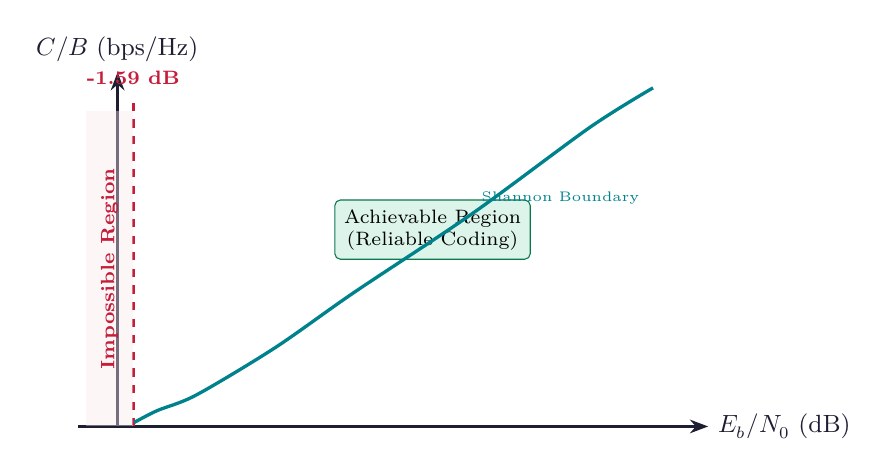
\begin{tikzpicture}
  % Draw axes
  \draw[-Stealth, thick, color=mydark] (-1.5,0) -- (6.5,0) node[right, font=\small] {$E_b/N_0$ (dB)};
  \draw[-Stealth, thick, color=mydark] (-1,0) -- (-1,4.5) node[above, font=\small] {$C/B$ (bps/Hz)};

  % Grid line for Shannon limit
  \draw[dashed, color=myred, line width=1pt] (-0.8,0) -- (-0.8,4.2) node[above, font=\scriptsize\bfseries\color{myred}] {-1.59 dB};

  % Draw shading for regions
  \fill[hdrred, opacity=0.4] (-1.4,0) rectangle (-0.8,4);
  \node[rotate=90, font=\scriptsize\bfseries\color{myred}] at (-1.1,2) {Impossible Region};
  \node[draw=mygreen, fill=hdrgreen, rounded corners=2pt, font=\scriptsize, align=center] at (3,2.5) {Achievable Region\\(Reliable Coding)};

  % Plot Shannon capacity limit curve
  % Coordinates scaled: dB = -1.6 -> x=-0.8, dB=0 -> x=0.5, dB=5 -> x=2.5, dB=10 -> x=5.0
  % C/B = 0 -> y=0, C/B = 1 -> y=1, C/B = 2 -> y=2.2, C/B = 4 -> y=3.8
  \draw[very thick, color=myteal, smooth] plot coordinates {
    (-0.79, 0.05) (-0.5, 0.2) (0.0, 0.4) (1.0, 1.0) (2.0, 1.7) (3.5, 2.7) (5.0, 3.8) (5.8, 4.3)
  };

  \node[right, font=\tiny\color{myteal}] at (3.5,2.9) {Shannon Boundary};
\end{tikzpicture}
\end{tcolorbox}

% ===============================================================================
% MANDATORY QUICK REVISION PAGE
% ===============================================================================
\newpage
\begin{center}
  {\large\bfseries\color{myred} Quick Revision --- Module II}\\[3pt]
  {\small\color{mydark} Markov Sources \& Channel Capacity $|$ PE-EC603D}
\end{center}
\noindent{\color{myred}\rule{\linewidth}{1.2pt}}
\vspace{4pt}

\begin{tcolorbox}[formulabox, title={\textbf{Key Formulas at a Glance}}]
\renewcommand{\arraystretch}{1.3}
\begin{tabularx}{\linewidth}{B{4.5cm} X}
Markov Transition Prob.  & $\sum_{j=1}^K p_{ij} = 1 \quad (\text{Row sum of TPM equals 1})$ \\[4pt]
Steady-State Vector     & $\mathbf{W}P = \mathbf{W} \quad \text{and} \quad \sum w_i = 1$ \\[4pt]
State Entropy           & $H_i = -\sum_{j=1}^K p_{ij} \log_2 p_{ij}$ \\[4pt]
Markov Source Entropy   & $H(X) = \sum w_i H_i$ \\[4pt]
Channel Capacity        & $C = \max_{P(x)} I(X;Y) \quad (\text{bits/channel-use})$ \\[4pt]
BSC Capacity            & $C_{\text{BSC}} = 1 - H(p) = 1 + p\log_2 p + (1-p)\log_2(1-p)$ \\[4pt]
BEC Capacity            & $C_{\text{BEC}} = 1 - \alpha$ \\[4pt]
Shannon-Hartley Theorem & $C = B \log_2 \left( 1 + \frac{S}{N} \right) = B \log_2 \left( 1 + \frac{S}{N_0 B} \right)$ (bps) \\[4pt]
Infinite Bandwidth Limit & $C_{\infty} = 1.44 \frac{S}{N_0}$ \\[4pt]
Shannon Limit (Min SNR) & $\left(\frac{E_b}{N_0}\right)_{\text{min}} = \ln 2 \approx 0.693 \approx -1.59 \text{ dB}$
\end{tabularx}
\end{tcolorbox}

\begin{tcolorbox}[defbox, title={\textbf{One-Line Definitions}}]
\begin{itemize}[leftmargin=*, itemsep=2.5pt, topsep=0pt]
  \item \textbf{Markov Source:} A source with memory where current output statistics depend on previous state history.
  \item \textbf{Transition Matrix (TPM):} A matrix storing conditional probabilities of moving between Markov states.
  \item \textbf{Steady-State Vector:} Stationary probabilities indicating long-run occupancy rates of Markov states.
  \item \textbf{Channel Capacity:} The maximum rate of information transmission that can be achieved over a channel.
  \item \textbf{Binary Symmetric Channel:} A binary channel model with symmetric error (crossover) probability $p$.
  \item \textbf{Binary Erasure Channel:} A channel model where bits are either received correctly or recognized as lost (erased).
  \item \textbf{AWGN Channel:} A continuous channel model corrupted by additive white Gaussian noise.
  \item \textbf{Shannon Limit:} The absolute minimum value of $E_b/N_0$ ($-1.59\text{ dB}$) required for error-free transmission.
\end{itemize}
\end{tcolorbox}

\begin{tcolorbox}[exambox, title={\textbf{Frequently Asked / Viva Questions}}]
\begin{enumerate}[topsep=0pt, label=\textbf{Q\arabic*.}, itemsep=5pt]
  \item \Q{State the main condition that defines a first-order Markov source.}
    The output probability at any time instant depends only on the output symbol of the immediately preceding time instant.
  \item \Q{Why does the sum of transition probabilities in each row of a TPM equal 1?}
    A row represents all transition possibilities leaving a specific state. The source must transition to one of the possible states, so the sum of these probabilities is certain (1).
  \item \Q{Explain the physical meaning of Shannon's Second Theorem.}
    If transmission rate $R \le C$, error-free communication is possible using coding. If $R > C$, it is physically impossible to achieve error-free communication.
  \item \Q{What happens to the capacity of a BSC when the crossover probability $p = 0.5$?}
    Capacity $C = 1 - H(0.5) = 1 - 1 = 0$. The channel output is completely random and independent of input, meaning no information can be transmitted.
  \item \Q{What is an "erasure" symbol in the context of a BEC?}
    It is a symbol received as a lost bit (labeled '$e$'), meaning the receiver knows a bit was sent but cannot determine if it was '0' or '1'.
  \item \Q{What are the components of noise in the Shannon-Hartley theorem?}
    Additive (noise is added to signal), White (flat power spectral density across all frequencies), and Gaussian (probability density function of noise voltage is Gaussian).
  \item \Q{Why can't we achieve infinite channel capacity by making the bandwidth infinite?}
    As bandwidth increases, the noise power $N = N_0 B$ also increases. The capacity reaches a thermodynamic limit of $1.44 S/N_0$ bps.
  \item \Q{Explain the bandwidth-SNR trade-off using a practical example.}
    In telephone channels with small bandwidth, high SNR is used to achieve high rates. In satellite links with low power (low SNR), wide bandwidths are used.
  \item \Q{State the value of the Shannon Limit and its practical significance.}
    $-1.59 \text{ dB}$. It is the absolute minimum signal-to-noise ratio per bit required to transmit information over an AWGN channel without errors.
  \item \Q{Under what conditions does the capacity of a channel equal its bandwidth?}
    When the signal-to-noise ratio $S/N = 1$ (or $0 \text{ dB}$), because $C = B \log_2(1+1) = B \log_2(2) = B$ bps.
  \item \Q{Distinguish between a lossless channel and a noiseless channel.}
    In a lossless channel, $H(Y|X) = 0$ (no noise, inputs map uniquely to outputs). In a noiseless channel, $H(X|Y) = 0$ (outputs map uniquely to inputs, no ambiguity).
  \item \Q{How do you calculate the entropy of a Markov source?}
    First, find steady-state probabilities $\mathbf{W}$. Then, calculate state entropies $H_i$. The average source entropy is the weighted sum $H(X) = \sum w_i H_i$.
\end{enumerate}
\tcbset{colbacktitle=mypurple, coltitle=white}
\end{tcolorbox}

\begin{tcolorbox}[tikzbox, title={Comparison of BSC and BEC Models}]
\renewcommand{\arraystretch}{1.45}
\par\noindent
\begin{tabularx}{\linewidth}{|B{3.2cm}|Y|Y|}
\hline
\textbf{Parameter} & \textbf{\color{myteal}Binary Symmetric Channel (BSC)} & \textbf{\color{mygreen}Binary Erasure Channel (BEC)} \\
\hline
\textbf{Input Alphabet} & Binary: $\{0, 1\}$ & Binary: $\{0, 1\}$ \\
\hline
\textbf{Output Alphabet} & Binary: $\{0, 1\}$ & Ternary: $\{0, e, 1\}$ (where $e$ is erasure) \\
\hline
\textbf{Error Type} & Bit flip (crossover), $0 \leftrightarrow 1$. & Bit loss, input becomes unreadable symbol $e$. \\
\hline
\textbf{Error Knowledge} & Receiver does not know which bits are flipped. & Receiver knows exactly which bits are erased. \\
\hline
\textbf{Capacity Formula} & $C = 1 - H(p)$ bits/use & $C = 1 - \alpha$ bits/use \\
\hline
\end{tabularx}
\end{tcolorbox}


% -- Module 3 -----------------------------------------------------------------
\modulestart{3}{Huffman Coding}

\section{Huffman Coding}
% ===============================================================================

Huffman coding is an optimal source coding technique used for lossy/lossless data compression. It belongs to the class of prefix-free codes, which are uniquely detectable.

\subsection{Definition and Concept}
\begin{tcolorbox}[defbox]
\textbf{Huffman Coding:} A bottom-up, variable-length source coding algorithm that assigns binary codes to symbols based on their probabilities. High-probability symbols are assigned shorter codewords, and low-probability symbols are assigned longer codewords, minimizing average codeword length.
\end{tcolorbox}

\subsection{The Huffman Coding Algorithm}
\begin{enumerate}[label=\textbf{Step \arabic*:}, leftmargin=4.5em, itemsep=3.5pt]
  \item Sort the source symbols in descending order of their probabilities.
  \item Combine the two lowest-probability symbols into a single node (parent node) with a probability equal to the sum of their probabilities.
  \item Assign binary '0' to one branch of the pair (usually the upper/higher probability branch) and '1' to the other branch.
  \item Place the combined node back into the list and re-sort all items in descending order.
  \item Repeat Steps 2 to 4 recursively until only one root node (probability = 1.0) remains.
  \item The codeword for each symbol is read by tracing the path from the root of the tree down to the symbol leaf node.
\end{enumerate}

\begin{tcolorbox}[examplebox, title={Worked Example: Huffman Coding}]
\textbf{Problem:} A discrete source emits 5 symbols $\{s_1, s_2, s_3, s_4, s_5\}$ with probabilities $P = \{0.4, 0.2, 0.2, 0.1, 0.1\}$.
\begin{enumerate}[label=\alph*., leftmargin=*, itemsep=1pt, topsep=1pt]
  \item Construct the Huffman code tree and determine the codewords.
  \item Calculate the average codeword length $L$ and coding efficiency $\eta$.
\end{enumerate}
\textbf{Solution:}

\textbf{(a) Tree Construction and Codewords:}
Tracing from the lowest probabilities up (bottom-up merging):
\begin{itemize}[leftmargin=*, itemsep=1pt]
  \item Merge $s_4$ (0.1) and $s_5$ (0.1) to create node $N_1$ with probability $0.2$. Assign 0 to $s_4$ and 1 to $s_5$.
  \item We now have nodes with probabilities $\{0.4, 0.2, 0.2, 0.2\}$. Merge the two lowest, say $s_3$ (0.2) and $N_1$ (0.2) to create $N_2$ with probability $0.4$. Assign 0 to $s_3$ and 1 to $N_1$.
  \item We now have $\{0.4, 0.4, 0.2\}$. Merge $s_2$ (0.2) and $N_2$ (0.4) to create $N_3$ with probability $0.6$. Assign 0 to $s_2$ and 1 to $N_2$.
  \item Merge $s_1$ (0.4) and $N_3$ (0.6) to create the root (1.0). Assign 0 to $s_1$ and 1 to $N_3$.
\end{itemize}

\begin{tabularx}{\linewidth}{|B{1.6cm}|Y|Y|B{1.8cm}|}
\hline
\textbf{Symbol} & \textbf{Probability ($P_i$)} & \textbf{Codeword Path} & \textbf{Length ($l_i$)} \\
\hline
$s_1$ & 0.4 & 0 & 1 \\
$s_2$ & 0.2 & 10 & 2 \\
$s_3$ & 0.2 & 110 & 3 \\
$s_4$ & 0.1 & 1110 & 4 \\
$s_5$ & 0.1 & 1111 & 4 \\
\hline
\end{tabularx}

\textbf{(b) Calculations:}
Source Entropy $H(X)$:
\begin{align*}
  H(X) &= -[0.4\log_2 0.4 + 2 \times (0.2\log_2 0.2) + 2 \times (0.1\log_2 0.1)] \\
  &= -[0.4(-1.3219) + 0.4(-2.3219) + 0.2(-3.3219)] \\
  &= -[-0.5288 - 0.9288 - 0.6644] = 2.122 \text{ bits/symbol}
\end{align*}
Average Codeword Length $L$:
\begin{align*}
  L &= \sum P_i l_i = (0.4 \times 1) + (0.2 \times 2) + (0.2 \times 3) + (0.1 \times 4) + (0.1 \times 4) \\
  &= 0.4 + 0.4 + 0.6 + 0.4 + 0.4 = 2.2 \text{ bits/symbol} \\[4pt]
  \text{Efficiency } \eta &= \frac{H(X)}{L} = \frac{2.122}{2.2} \times 100\% = 96.45\%
\end{align*}
\end{tcolorbox}

\begin{tcolorbox}[tikzbox, title={Huffman Coding Tree Diagram}]
\centering
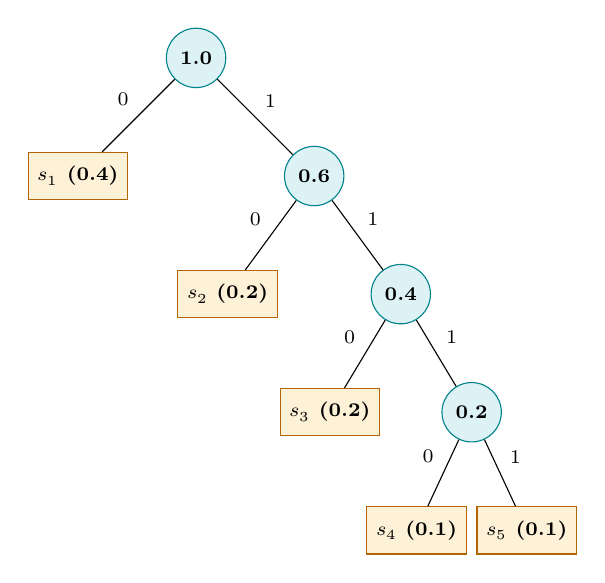
\begin{tikzpicture}[level distance=1.5cm,
  level 1/.style={sibling distance=3.0cm},
  level 2/.style={sibling distance=2.2cm},
  level 3/.style={sibling distance=1.8cm},
  level 4/.style={sibling distance=1.4cm},
  tnode/.style={circle, draw=myteal, fill=hdrteal, minimum size=0.6cm, font=\scriptsize\bfseries},
  leaf/.style={rectangle, draw=myamber, fill=hdramber, minimum size=0.6cm, font=\scriptsize\bfseries}]

  \node[tnode] (root) {1.0}
    child {node[leaf] (s1) {$s_1$ (0.4)}
      edge from parent node[above left, font=\scriptsize] {0}
    }
    child {node[tnode] (n3) {0.6}
      child {node[leaf] (s2) {$s_2$ (0.2)}
        edge from parent node[above left, font=\scriptsize] {0}
      }
      child {node[tnode] (n2) {0.4}
        child {node[leaf] (s3) {$s_3$ (0.2)}
          edge from parent node[above left, font=\scriptsize] {0}
        }
        child {node[tnode] (n1) {0.2}
          child {node[leaf] (s4) {$s_4$ (0.1)}
            edge from parent node[above left, font=\scriptsize] {0}
          }
          child {node[leaf] (s5) {$s_5$ (0.1)}
            edge from parent node[above right, font=\scriptsize] {1}
          }
          edge from parent node[above right, font=\scriptsize] {1}
        }
        edge from parent node[above right, font=\scriptsize] {1}
      }
      edge from parent node[above right, font=\scriptsize] {1}
    };
\end{tikzpicture}
\end{tcolorbox}

% ===============================================================================
\section{Cyclic Codes}
% ===============================================================================

Channel coding techniques inject structured redundancy into data packets to allow detection and correction of channel-induced errors.

\subsection{Definition of Cyclic Codes}
\begin{tcolorbox}[defbox]
\textbf{Cyclic Code:} A linear block code $(n, k)$ with the algebraic property that any cyclic shift of a valid codeword is also a valid codeword.
\par\vspace{3pt}
If $C = (c_0, c_1, \dots, c_{n-1})$ is a codeword, then $C^{(1)} = (c_{n-1}, c_0, \dots, c_{n-2})$ is also a codeword.
\end{tcolorbox}

In polynomial representation, a codeword is represented as:
\begin{equation}
  c(x) = c_0 + c_1 x + c_2 x^2 + \dots + c_{n-1} x^{n-1}
\end{equation}
The cyclic shift property means that if $c(x)$ is a codeword, then the remainder of $x c(x)$ divided by $x^n + 1$ is also a codeword.

\subsection{Generator Polynomial $g(x)$}
Every cyclic code is uniquely defined by a **generator polynomial** $g(x)$ of degree $n-k$.
\begin{itemize}[leftmargin=*, itemsep=2pt]
  \item $g(x)$ must be a factor of the polynomial $x^n + 1$ over GF(2) (Galois Field of 2, modulo-2 arithmetic).
  \item A polynomial $c(x)$ of degree $\le n-1$ is a valid codeword if and only if it is a multiple of $g(x)$:
    \begin{equation}
      c(x) = m(x) \cdot g(x)
    \end{equation}
    Where $m(x)$ is the message polynomial of degree $\le k-1$.
\end{itemize}

\subsection{Systematic Encoding of Cyclic Codes}
In systematic codes, the first $k$ bits represent the message directly, and the remaining $n-k$ bits are parity check bits.
\begin{tcolorbox}[formulabox, title={\textbf{Systematic Cyclic Coding Steps}}]
For message polynomial $m(x)$ and generator polynomial $g(x)$ of degree $n-k$:
\begin{enumerate}[label=\textbf{Step \arabic*:}, leftmargin=4.5em, itemsep=2pt, topsep=1pt]
  \item Multiply the message polynomial by $x^{n-k}$:
    \begin{equation*}
      u(x) = x^{n-k} m(x)
    \end{equation*}
  \item Divide $u(x)$ by $g(x)$ to obtain the remainder polynomial $r(x)$:
    \begin{equation*}
      \frac{x^{n-k} m(x)}{g(x)} = q(x) + \frac{r(x)}{g(x)} \implies r(x) = \text{rem}\left[ \frac{x^{n-k} m(x)}{g(x)} \right]
    \end{equation*}
  \item Form the codeword polynomial $c(x)$ by adding the remainder $r(x)$ to $u(x)$ (addition is XOR in GF(2)):
    \begin{equation}
      c(x) = x^{n-k} m(x) + r(x)
    \end{equation}
\end{enumerate}
\end{tcolorbox}

\begin{tcolorbox}[examplebox, title={Worked Example: (7, 4) Cyclic Systematic Code}]
\textbf{Problem:} For a $(7, 4)$ cyclic code, the generator polynomial is $g(x) = x^3 + x + 1$. Encode the message vector $m = [1, 0, 1, 1]$ systematically.\\[4pt]
\textbf{Solution:}
Identify parameters: $n=7$, $k=4$, $n-k=3$.
Convert message vector to polynomial:
\begin{equation*}
  m(x) = 1 \cdot x^0 + 0 \cdot x^1 + 1 \cdot x^2 + 1 \cdot x^3 = 1 + x^2 + x^3
\end{equation*}
Multiply $m(x)$ by $x^{n-k} = x^3$:
\begin{equation*}
  x^3 m(x) = x^3 (1 + x^2 + x^3) = x^3 + x^5 + x^6
\end{equation*}
Divide $x^3 m(x)$ by $g(x) = x^3 + x + 1$ using modulo-2 long division:
\begin{align*}
  &\text{Divide: } x^6 + x^5 + x^3 \text{ by } x^3 + x + 1 \\
  &x^6 + x^5 + x^3 = x^3(x^3 + x + 1) + x^5 + x^4 \quad (\text{since } x^6+x^4+x^3 \text{ subtracted leaves } x^5+x^4) \\
  &\text{Continuing long division gives: } \\
  &x^3 + x + 1 \overline{) x^6 + x^5 + 0x^4 + x^3} \\
  &\phantom{x^3 + x + 1} \underline{x^6 + 0x^5 + x^4 + x^3} \quad (\text{multiply by } x^3) \\
  &\phantom{x^3 + x + 1} \phantom{x^6 + } x^5 + x^4 + 0x^3 \\
  &\phantom{x^3 + x + 1} \phantom{x^6 + } \underline{x^5 + 0x^4 + x^3 + x^2} \quad (\text{multiply by } x^2) \\
  &\phantom{x^3 + x + 1} \phantom{x^6 + x^5 + } x^4 + x^3 + x^2 \\
  &\phantom{x^3 + x + 1} \phantom{x^6 + x^5 + } \underline{x^4 + 0x^3 + x^2 + x} \quad (\text{multiply by } x) \\
  &\phantom{x^3 + x + 1} \phantom{x^6 + x^5 + x^4 + } x^3 + 0x^2 + x \\
  &\phantom{x^3 + x + 1} \phantom{x^6 + x^5 + x^4 + } \underline{x^3 + 0x^2 + x + 1} \quad (\text{multiply by } 1) \\
  &\phantom{x^3 + x + 1} \phantom{x^6 + x^5 + x^4 + x^3 + } 1 \quad (\text{Remainder})
\end{align*}
Thus, the remainder is $r(x) = 1$.
Construct the codeword:
\begin{align*}
  c(x) &= x^3 m(x) + r(x) = (x^6 + x^5 + x^3) + 1 = 1 + x^3 + x^5 + x^6
\end{align*}
Convert polynomial to codeword vector:
\begin{equation*}
  C = [1, 0, 0, 1, 0, 1, 1]
\end{equation*}
Where the first 3 bits $[1, 0, 0]$ represent the parity check bits, and the last 4 bits $[1, 0, 1, 1]$ represent the message.
\end{tcolorbox}

\subsection{Hardware Encoder using Feedback Shift Registers (FSR)}
Cyclic codes are popular because their encoding and syndrome circuits can be implemented efficiently in hardware using shift registers and XOR gates (modulo-2 adders).

\begin{tcolorbox}[tikzbox, title={Feedback Shift Register Encoder for $g(x) = x^3 + x + 1$}]
\centering
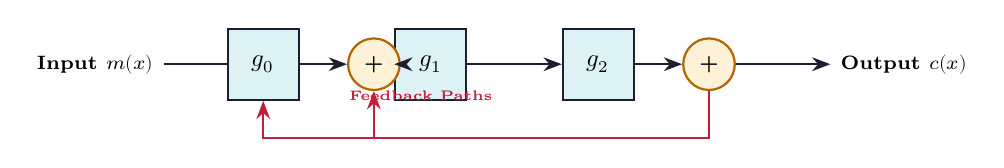
\begin{tikzpicture}[node distance=1.2cm, thick]
  % Draw registers
  \node[rectangle, draw=mydark, fill=hdrteal, minimum size=0.9cm, font=\small\bfseries] (R0) {$g_0$};
  \node[rectangle, draw=mydark, fill=hdrteal, minimum size=0.9cm, right=1.2cm of R0, font=\small\bfseries] (R1) {$g_1$};
  \node[rectangle, draw=mydark, fill=hdrteal, minimum size=0.9cm, right=1.2cm of R1, font=\small\bfseries] (R2) {$g_2$};

  % XOR sum junction (modulo 2 addition)
  \node[circle, draw=myamber, fill=hdramber, minimum size=0.5cm, right=0.6cm of R0, font=\scriptsize\bfseries] (xor1) {+};
  \node[circle, draw=myamber, fill=hdramber, minimum size=0.5cm, right=0.6cm of R2, font=\scriptsize\bfseries] (xor2) {+};

  % Input & Output
  \node (in) [left=0.8cm of R0, font=\scriptsize\bfseries] {Input $m(x)$};
  \node (out) [right=1.2cm of xor2, font=\scriptsize\bfseries] {Output $c(x)$};

  % Inter-register wires
  \draw[arrow] (R0) -- (xor1);
  \draw[arrow] (xor1) -- (R1);
  \draw[arrow] (R1) -- (R2);
  \draw[arrow] (R2) -- (xor2);
  \draw[arrow] (xor2) -- (out);

  % Feedback paths
  \draw[line] (in) -- (R0);
  \draw[redarrow] (xor2.south) -- ++(0,-0.6) -| (xor1.south);
  \draw[redarrow] (xor2.south) -- ++(0,-0.6) -| (R0.south);
  
  \node[font=\tiny\bfseries\color{myred}] at (2.0, -0.4) {Feedback Paths};
\end{tikzpicture}
\end{tcolorbox}

% ===============================================================================
\section{Convolutional Codes}
% ===============================================================================

Linear block codes processes data block-by-block. **Convolutional codes**, in contrast, process information continuously, using internal shift-register states to create memory dependencies.

\subsection{Basic Principles and Structure}
A convolutional encoder is defined by three parameters $(n, k, K)$:
\begin{itemize}[leftmargin=*, itemsep=2pt]
  \item $n$: Number of output bits produced in each shift cycle.
  \item $k$: Number of input bits processed in each shift cycle.
  \item $K$: Constraint length (number of shift register stages that affect the output).
\end{itemize}
The code rate is defined as $r = k/n$. The outputs are computed by modulo-2 addition of the current input and the values stored in the shift registers.

\begin{tcolorbox}[tikzbox, title={Convolutional Encoder Circuit (Rate $1/2$, Constraint Length $K=3$)}]
\centering
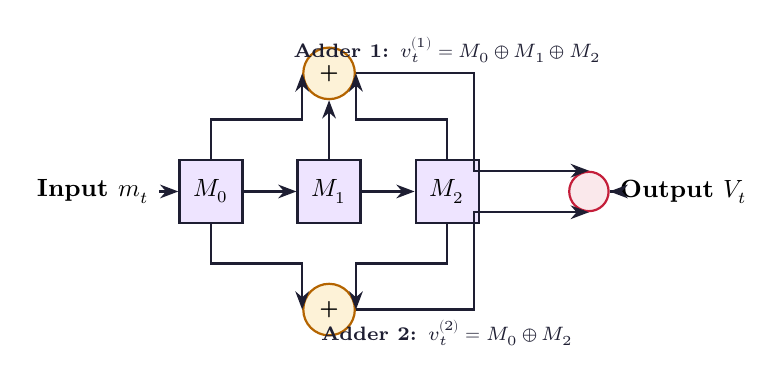
\begin{tikzpicture}[node distance=1.0cm, thick]
  % Input
  \node (in) at (-1.5, 0) [font=\small\bfseries] {Input $m_t$};

  % Shift Registers
  \node[rectangle, draw=mydark, fill=hdrpurple, minimum width=0.8cm, minimum height=0.8cm, font=\small\bfseries] (S0) at (0, 0) {$M_0$};
  \node[rectangle, draw=mydark, fill=hdrpurple, minimum width=0.8cm, minimum height=0.8cm, font=\small\bfseries] (S1) at (1.5, 0) {$M_1$};
  \node[rectangle, draw=mydark, fill=hdrpurple, minimum width=0.8cm, minimum height=0.8cm, font=\small\bfseries] (S2) at (3.0, 0) {$M_2$};

  % Modulo-2 adders (XOR)
  \node[circle, draw=myamber, fill=hdramber, minimum size=0.55cm, font=\scriptsize\bfseries] (xor1) at (1.5, 1.5) {+};
  \node[circle, draw=myamber, fill=hdramber, minimum size=0.55cm, font=\scriptsize\bfseries] (xor2) at (1.5, -1.5) {+};

  % Output selector switch
  \node[circle, draw=myred, fill=hdrred, minimum size=0.5cm] (sw) at (4.8, 0) {};
  \node (out) at (6.0, 0) [font=\small\bfseries] {Output $V_t$};

  % Connections
  \draw[arrow] (in) -- (S0);
  \draw[arrow] (S0) -- (S1);
  \draw[arrow] (S1) -- (S2);

  % Wires to XOR 1 (Upper Adder)
  \draw[arrow] (S0.north) -- ++(0,0.5) -| (xor1.west);
  \draw[arrow] (S1.north) -- (xor1.south);
  \draw[arrow] (S2.north) -- ++(0,0.5) -| (xor1.east);

  % Wires to XOR 2 (Lower Adder)
  \draw[arrow] (S0.south) -- ++(0,-0.5) -| (xor2.west);
  \draw[arrow] (S2.south) -- ++(0,-0.5) -| (xor2.east);

  % Output switch routing
  \draw[arrow] (xor1.east) -- ++(1.5,0) |- (sw.north);
  \draw[arrow] (xor2.east) -- ++(1.5,0) |- (sw.south);
  \draw[arrow] (sw) -- (out);

  % Labels
  \node[font=\scriptsize\bfseries\color{mydark}] at (3.0, 1.8) {Adder 1: $v^{(1)}_t = M_0 \oplus M_1 \oplus M_2$};
  \node[font=\scriptsize\bfseries\color{mydark}] at (3.0, -1.8) {Adder 2: $v^{(2)}_t = M_0 \oplus M_2$};
\end{tikzpicture}
\end{tcolorbox}

\subsection{Representations of Convolutional Codes}
Three graphical methods are used to describe a convolutional code:
\begin{enumerate}[label=\textbf{\arabic*.}, leftmargin=*, itemsep=3pt]
  \item \textbf{State Diagram:} Shows the states of the shift registers (excluding the current input) and the transitions between states caused by input '0' or '1'.
  \item \textbf{Tree Diagram:} Shows all possible output paths as a branching tree structure, where the path branches upward for input '0' and downward for input '1'.
  \item \textbf{Trellis Diagram:} A time-extended state transition diagram. It lists all possible states vertically at each time step, and shows transitions horizontally.
\end{enumerate}

\begin{tcolorbox}[tikzbox, title={Trellis Diagram Transition Segment}]
\centering
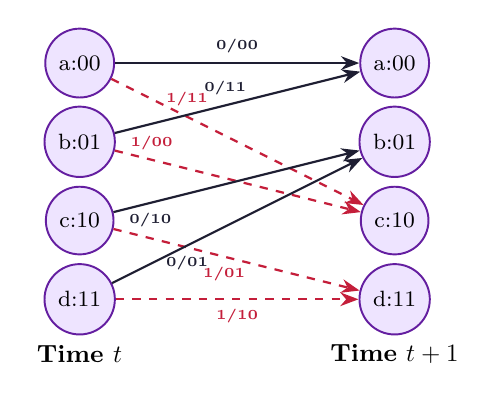
\begin{tikzpicture}[node distance=1.5cm, thick]
  % Define states at time t
  \node[snode] (a_t) at (0, 3) {a:00};
  \node[snode] (b_t) at (0, 2) {b:01};
  \node[snode] (c_t) at (0, 1) {c:10};
  \node[snode] (d_t) at (0, 0) {d:11};

  % Define states at time t+1
  \node[snode] (a_t1) at (4, 3) {a:00};
  \node[snode] (b_t1) at (4, 2) {b:01};
  \node[snode] (c_t1) at (4, 1) {c:10};
  \node[snode] (d_t1) at (4, 0) {d:11};

  % Transitions from state 'a' (input 0 -> solid; input 1 -> dashed)
  \draw[arrow] (a_t) -- (a_t1) node[midway, above, font=\tiny\bfseries] {0/00};
  \draw[arrow, dashed, color=myred] (a_t) -- (c_t1) node[pos=0.3, above, font=\tiny\bfseries\color{myred}] {1/11};

  % Transitions from state 'b'
  \draw[arrow] (b_t) -- (a_t1) node[pos=0.45, above, font=\tiny\bfseries] {0/11};
  \draw[arrow, dashed, color=myred] (b_t) -- (c_t1) node[pos=0.15, above, font=\tiny\bfseries\color{myred}] {1/00};

  % Transitions from state 'c'
  \draw[arrow] (c_t) -- (b_t1) node[pos=0.15, below, font=\tiny\bfseries] {0/10};
  \draw[arrow, dashed, color=myred] (c_t) -- (d_t1) node[pos=0.45, below, font=\tiny\bfseries\color{myred}] {1/01};

  % Transitions from state 'd'
  \draw[arrow] (d_t) -- (b_t1) node[pos=0.3, below, font=\tiny\bfseries] {0/01};
  \draw[arrow, dashed, color=myred] (d_t) -- (d_t1) node[midway, below, font=\tiny\bfseries\color{myred}] {1/10};

  % Time step indicators
  \node at (0, -0.7) [font=\small\bfseries] {Time $t$};
  \node at (4, -0.7) [font=\small\bfseries] {Time $t+1$};
\end{tikzpicture}
\end{tcolorbox}

\subsection{Viterbi Decoding Algorithm}
The Viterbi algorithm is the standard decoding method for convolutional codes. It finds the most likely sequence of transmitted symbols (minimum Hamming distance path) through the trellis.
\begin{itemize}[leftmargin=*, itemsep=3.5pt]
  \item \textbf{Branch Metric:} The Hamming distance between the received bits and the expected output bits for a specific branch.
  \item \textbf{Path Metric:} The accumulated sum of branch metrics along a path.
  \item \textbf{Survivor Path:} At each node in the trellis, the incoming path with the lowest path metric is saved, and all other paths are discarded. This prevents exponential path growth.
\end{itemize}

% ===============================================================================
\section{Arithmetic Coding}
% ===============================================================================

Huffman coding assigns an integer number of bits to each symbol. If a symbol has a probability of $0.9$, its ideal code length is $-\log_2 0.9 \approx 0.15$ bits, but Huffman must assign at least 1 bit, reducing efficiency. **Arithmetic coding** overcomes this constraint.

\subsection{Core Concept}
\begin{tcolorbox}[defbox]
\textbf{Arithmetic Coding:} A non-block source coding algorithm that maps an entire sequence of symbols to a single fractional number in the interval $[0, 1)$. Symbols are represented by ranges proportional to their probabilities.
\end{tcolorbox}

\subsection{Encoding Procedure}
\begin{enumerate}[label=\textbf{Step \arabic*:}, leftmargin=4.5em, itemsep=2pt, topsep=1pt]
  \item Initialize the interval boundaries: $\text{Low} = 0$, $\text{High} = 1$.
  \item For each symbol in the message:
    \begin{align}
      \text{Range} &= \text{High} - \text{Low} \\
      \text{High} &= \text{Low} + \text{Range} \times \text{Upper\_Cum\_Prob}(s_i) \\
      \text{Low} &= \text{Low} + \text{Range} \times \text{Lower\_Cum\_Prob}(s_i)
    \end{align}
  \item Repeat for all symbols in the sequence.
  \item The final output is any floating-point number within the final $[\text{Low}, \text{High})$ interval.
\end{enumerate}

\begin{tcolorbox}[examplebox, title={Worked Example: Arithmetic Coding of "WET"}]
\textbf{Problem:} A source has three symbols $\{E, T, W\}$ with probabilities $\{0.5, 0.3, 0.2\}$.
\begin{enumerate}[label=\alph*., leftmargin=*, itemsep=1pt, topsep=1pt]
  \item Calculate the cumulative probability ranges for the symbols.
  \item Encode the sequence "WET".
\end{enumerate}
\textbf{Solution:}

\textbf{(a) Probability Ranges:}\par\noindent
Sort alphabet (say alphabetically $\{E, T, W\}$):
\begin{itemize}[leftmargin=*, itemsep=1pt]
  \item Symbol $E$ (prob = 0.5): Cumulative Interval $[0.0, 0.5)$
  \item Symbol $T$ (prob = 0.3): Cumulative Interval $[0.5, 0.8)$
  \item Symbol $W$ (prob = 0.2): Cumulative Interval $[0.8, 1.0)$
\end{itemize}

\textbf{(b) Encode "WET":}
\begin{itemize}[leftmargin=*, itemsep=3pt]
  \item \textbf{Initial State:} $\text{Low} = 0$, $\text{High} = 1$, $\text{Range} = 1.0$.
  \item \textbf{First Symbol: 'W'} (Sub-interval $[0.8, 1.0)$):
    \begin{align*}
      \text{Low} &= 0 + 1.0 \times 0.8 = 0.8 \\
      \text{High} &= 0 + 1.0 \times 1.0 = 1.0 \\
      \text{Range} &= 1.0 - 0.8 = 0.2
    \end{align*}
  \item \textbf{Second Symbol: 'E'} (Sub-interval $[0.0, 0.5)$ relative to current range):
    \begin{align*}
      \text{Low} &= 0.8 + 0.2 \times 0.0 = 0.8 \\
      \text{High} &= 0.8 + 0.2 \times 0.5 = 0.9 \\
      \text{Range} &= 0.9 - 0.8 = 0.1
    \end{align*}
  \item \textbf{Third Symbol: 'T'} (Sub-interval $[0.5, 0.8)$ relative to current range):
    \begin{align*}
      \text{Low} &= 0.8 + 0.1 \times 0.5 = 0.85 \\
      \text{High} &= 0.8 + 0.1 \times 0.8 = 0.88 \\
      \text{Range} &= 0.88 - 0.85 = 0.03
    \end{align*}
\end{itemize}
The final interval is $[0.85, 0.88)$. Any number in this range (e.g., \textbf{0.86}) represents the sequence "WET".
\end{tcolorbox}

% ===============================================================================
% MANDATORY QUICK REVISION PAGE
% ===============================================================================
\newpage
\begin{center}
  {\large\bfseries\color{myred} Quick Revision --- Module III}\\[3pt]
  {\small\color{mydark} Source \& Channel Coding $|$ PE-EC603D}
\end{center}
\noindent{\color{myred}\rule{\linewidth}{1.2pt}}
\vspace{4pt}

\begin{tcolorbox}[formulabox, title={\textbf{Key Formulas at a Glance}}]
\renewcommand{\arraystretch}{1.3}
\begin{tabularx}{\linewidth}{B{4.5cm} X}
Average Codeword Length & $L = \sum P_i l_i \quad (\text{bits/symbol})$ \\[4pt]
Huffman Efficiency      & $\eta = \frac{H(X)}{L} \times 100\%$ \\[4pt]
Cyclic Shift Shift      & $C^{(1)} = (c_{n-1}, c_0, \dots, c_{n-2})$ \\[4pt]
Codeword Polynomial     & $c(x) = m(x) g(x) \quad (\text{Non-systematic})$ \\[4pt]
Systematic Codeword     & $c(x) = x^{n-k} m(x) + r(x) \quad$ where $r(x) = \text{rem}\left[\frac{x^{n-k} m(x)}{g(x)}\right]$ \\[6pt]
Syndrome Polynomial     & $s(x) = \text{rem}\left[\frac{r(x)}{g(x)}\right] \quad (\text{If } s(x)=0, \text{ no error})$ \\[4pt]
Convolutional Code Rate & $r = k/n$ \\[4pt]
Arithmetic Coding Range & $\text{Range} = \text{High} - \text{Low}$
\end{tabularx}
\end{tcolorbox}

\begin{tcolorbox}[defbox, title={\textbf{One-Line Definitions}}]
\begin{itemize}[leftmargin=*, itemsep=2.5pt, topsep=0pt]
  \item \textbf{Huffman Coding:} A bottom-up optimal variable-length source coding technique based on sorting and merging probabilities.
  \item \textbf{Cyclic Code:} A linear block code where any cyclic shift of a codeword is also a valid codeword.
  \item \textbf{Generator Polynomial:} A unique polynomial $g(x)$ of degree $n-k$ that generates all codewords of a cyclic code.
  \item \textbf{Syndrome:} A polynomial remainder computed by the decoder to detect and locate errors in cyclic codes.
  \item \textbf{Constraint Length ($K$):} The number of shift register stages affecting output bits in a convolutional encoder.
  \item \textbf{Trellis Diagram:} A time-indexed state diagram representing paths and state transitions in convolutional codes.
  \item \textbf{Viterbi Decoder:} A maximum likelihood decoding algorithm using trellis paths to find the survivor path.
  \item \textbf{Arithmetic Coding:} A non-block coding method mapping a sequence of symbols to a single fractional number in $[0, 1)$.
\end{itemize}
\end{tcolorbox}

\begin{tcolorbox}[exambox, title={\textbf{Frequently Asked / Viva Questions}}]
\begin{enumerate}[topsep=0pt, label=\textbf{Q\arabic*.}, itemsep=5pt]
  \item \Q{Why are Huffman codes uniquely decodable?}
    They possess the prefix-free property, meaning no codeword is a prefix of any other. This allows symbol-by-symbol decoding without ambiguity.
  \item \Q{What is the difference between systematic and non-systematic codes?}
    In systematic codes, the message bits appear unchanged at the beginning (or end) of the codeword. In non-systematic codes, message and parity bits are mixed.
  \item \Q{State the algebraic condition for a polynomial to be a generator polynomial of a cyclic code.}
    It must be of degree $n-k$ and must be a factor of $x^n + 1$ over Galois Field GF(2).
  \item \Q{How are parity bits calculated in systematic cyclic codes?}
    By dividing $x^{n-k} m(x)$ by $g(x)$ using modulo-2 division. The remainder of this division is the parity check polynomial $r(x)$.
  \item \Q{What hardware components are required to build a cyclic code encoder?}
    Linear Feedback Shift Registers (LFSRs) consisting of D flip-flops, XOR gates (modulo-2 adders), and switches.
  \item \Q{State the difference between block codes and convolutional codes.}
    Block codes process data in fixed, independent blocks. Convolutional codes process data continuously, utilizing internal register states to create memory dependencies.
  \item \Q{What parameters define a convolutional code?}
    $(n, k, K)$, where $n$ is output bits per cycle, $k$ is input bits per cycle, and $K$ is the constraint length.
  \item \Q{Explain the role of the Viterbi algorithm in convolutional decoding.}
    It acts as a maximum-likelihood decoder, finding the path through the trellis that minimizes the Hamming distance (or Euclidean distance) to the received sequence.
  \item \Q{What is a "survivor path" in Viterbi decoding?}
    At each trellis node, two paths enter. The path with the lower accumulated metric (errors) is kept as the survivor path, and the other is discarded.
  \item \Q{Why does arithmetic coding outperform Huffman coding for highly skewed probability sources?}
    Huffman requires an integer number of bits per symbol, causing inefficiency for symbols with probabilities $>0.5$. Arithmetic coding represents sequences as a single fraction.
  \item \Q{How does the receiver decode an arithmetic code?}
    The receiver uses the received fractional value to determine which symbol's sub-interval contains the value, outputs the symbol, updates the interval, and repeats.
  \item \Q{What is the relationship between the degree of $g(x)$ and cyclic code parameters?}
    The degree of the generator polynomial $g(x)$ is always equal to $n-k$, which is the number of parity check bits in the $(n, k)$ code.
\end{enumerate}
\tcbset{colbacktitle=mypurple, coltitle=white}
\end{tcolorbox}

\begin{tcolorbox}[tikzbox, title={Comparison of Coding Techniques}]
\renewcommand{\arraystretch}{1.45}
\par\noindent
\begin{tabularx}{\linewidth}{|B{3.2cm}|Y|Y|}
\hline
\textbf{Parameter} & \textbf{\color{myteal}Cyclic Codes} & \textbf{\color{mygreen}Convolutional Codes} \\
\hline
\textbf{Structure} & Block-based (processes blocks of length $k$). & Continuous (processes streams of bits). \\
\hline
\textbf{Memory} & Memoryless between blocks. & Memory-based (states of shift registers). \\
\hline
\textbf{Implementation} & LFSR shift registers and XOR gates. & Shift registers and modulo-2 adders. \\
\hline
\textbf{Decoding} & Syndrome calculations. & Trellis-based Viterbi decoding. \\
\hline
\textbf{Applications} & Error detection (CRC in Ethernet, USB). & Deep space communications, cellular (LTE). \\
\hline
\end{tabularx}
\end{tcolorbox}


\end{document}
